\documentclass[12pt,letterpaper]{article}

% =========================================================================
% PAQUETES FUNDAMENTALES
% =========================================================================
\usepackage[utf8]{inputenc}
\usepackage[spanish,es-tabla]{babel}
\usepackage[margin=2.54cm]{geometry}
\usepackage{amsmath, amssymb, amsfonts}
\usepackage{graphicx}
\usepackage{booktabs}
\usepackage{tabularx}
\usepackage{array}
\usepackage{multirow}
\usepackage{xcolor}
\usepackage{microtype}
\usepackage{setspace}
\usepackage{caption}
\usepackage{subcaption}

% Delimitadores de citas parentéticas según formato APA 7: (Autor, Año)
\makeatletter
\def\@cite#1#2{({#1\if@tempswa , #2\fi})}
\makeatother
\providecommand{\citep}[1]{\cite{#1}}
\providecommand{\citet}[1]{\cite{#1}}

% Configuración de Títulos de Tablas y Figuras según APA 7.ª Edición
\captionsetup[table]{
    position=above,
    labelsep=newline,
    justification=raggedright,
    singlelinecheck=false,
    labelfont=bf,
    textfont=it
}
\captionsetup[figure]{
    position=above,
    labelsep=newline,
    justification=raggedright,
    singlelinecheck=false,
    labelfont=bf,
    textfont=it
}

% =========================================================================
% TIKZ PARA DIAGRAMAS VECTORIALES (ÁRBOLES DE PROBLEMAS Y OBJETIVOS)
% =========================================================================
\usepackage{tikz}
\usetikzlibrary{arrows.meta, positioning, shapes.geometric, shadows, trees}

% =========================================================================
% HIPERVÍNCULOS Y METADATOS PDF
% =========================================================================
\usepackage{hyperref}
\hypersetup{
    colorlinks=true,
    linkcolor=blue!75!black,
    citecolor=green!50!black,
    urlcolor=cyan!70!black,
    pdfauthor={Julio Nelson Arias Cruz, Serrano Mamani Raquel Araceli, Mario Fabricio Murillo Peñaranda},
    pdftitle={Sistema de Contraste de Ingresos Operativos Declarados mediante Machine Learning},
    pdfsubject={Machine Learning DAT-255 - UMSA},
    pdfkeywords={Machine Learning, EAIMCS, INE Bolivia, Random Forest, Duan Smearing, Data Drift}
}

% =========================================================================
% INTERLINEADO Y ESPACIADO DE PÁRRAFOS (NORMAS APA 7 ESTRICTO)
% =========================================================================
\doublespacing % Interlineado doble estricto reglamentario según norma oficial APA 7.ª Edición
\setlength{\parindent}{1.27cm} % Sangría de primera línea reglamentaria de 0.5 pulgadas
\setlength{\parskip}{0pt}      % Sin separación adicional entre párrafos según estándar APA 7

% =========================================================================
% CUERPO DEL DOCUMENTO
% =========================================================================
\begin{document}

% -------------------------------------------------------------------------
% CARÁTULA OFICIAL
% -------------------------------------------------------------------------
\begin{titlepage}
    \centering
    \vspace*{0.2cm}
    
    {\fontsize{17pt}{22pt}\selectfont \textbf{UNIVERSIDAD MAYOR DE SAN ANDRÉS}}\\[0.25cm]
    {\fontsize{14pt}{18pt}\selectfont \textbf{FACULTAD DE CIENCIAS PURAS Y NATURALES}}\\[0.2cm]
    {\fontsize{13pt}{17pt}\selectfont \textbf{CARRERA DE INFORMÁTICA}}\\[0.2cm]
    {\fontsize{12pt}{16pt}\selectfont \textbf{MACHINE LEARNING DAT-255}}\\[0.8cm]
    
    % LOGO DE LA UNIVERSIDAD (Imagen o Vector TikZ elegante como fallback)
    \IfFileExists{imagenes/logo_umsa.png}{
        
\includegraphics[height=6cm,keepaspectratio]{imagenes/logo_umsa.png}
    }
    
    % TÍTULO DEL PROYECTO
    \rule{\linewidth}{1.2pt}\\[0.4cm]
    {\fontsize{15pt}{19pt}\selectfont \textbf{SISTEMA DE CONTRASTE DE INGRESOS OPERATIVOS DECLARADOS MEDIANTE MACHINE LEARNING}}
    \rule{\linewidth}{1.2pt}\\[0.1cm]
    
    % ESTUDIANTES, DOCENTE Y ENLACES INSTITUCIONALES DEL PROYECTO
    \begin{minipage}{0.94\textwidth}
        \fontsize{10pt}{14.5pt}\selectfont
        \begin{tabular}{ll}
            \textbf{ESTUDIANTES:} & Julio Nelson Arias Cruz \\
                                  & Serrano Mamani Raquel Araceli \\
                                  & Mario Fabricio Murillo Peñaranda \\[0.35cm]
            \textbf{DOCENTE:}     & M. Sc. Menfy Morales Rios \\[0.35cm]
            \textbf{PLATAFORMA WEB:} & \url{https://finalprojectml.onrender.com/} \\[0.18cm]
            \textbf{PROYECTO EN GITHUB:}      & \url{https://github.com/JulioArias7200/finalProjectML} \\
        \end{tabular}
    \end{minipage}
    
    \vfill
    
    {\fontsize{11pt}{14pt}\selectfont \textbf{La Paz -- Bolivia}}\\[0.05cm]
    {\fontsize{10pt}{12pt}\selectfont 2026}
\end{titlepage}

% -------------------------------------------------------------------------
% ÍNDICES
% -------------------------------------------------------------------------
\pagenumbering{roman}
\tableofcontents
\newpage
\listoffigures
\vspace{1cm}
\listoftables
\newpage

\pagenumbering{arabic}
\setcounter{page}{1}

% -------------------------------------------------------------------------
% SECCIONES MODULARES DEL INFORME
% -------------------------------------------------------------------------
\section{Introducción}
\label{sec:introduccion}

En el ámbito de la macroeconomía aplicada y la administración pública moderna, la consolidación de estadísticas confiables de Cuentas Nacionales y el aseguramiento de la equidad tributaria representan pilares esenciales para el diseño de políticas públicas orientadas al desarrollo socioeconómico sostenible. En el Estado Plurinacional de Bolivia, el Instituto Nacional de Estadística (INE) ejecuta periódicamente censos y encuestas sectoriales con el fin de cuantificar el desempeño de las unidades económicas y calcular agregados macroeconómicos fundamentales, tales como el Producto Interno Bruto (PIB) por el enfoque de la producción y la formación bruta de capital fijo.

Entre estas operaciones estadísticas, la \textit{Encuesta a la Industria Manufacturera, Comercio y Servicios} (EAIMCS), referenciada en el catálogo oficial ANDA bajo el código \texttt{BOL-INE-}\allowbreak\texttt{EAIMCS-}\allowbreak\texttt{2017-2018}, constituye una de las fuentes de información microeconómica más exhaustivas del país para el estrato de medianas y grandes empresas. A través de cuestionarios especializados, la EAIMCS recopila datos detallados sobre la dotación de mano de obra, remuneraciones salariales, consumo de materias primas, gastos energéticos, capacidad física instalada y valor histórico de los activos fijos.

No obstante, tanto las autoridades estadísticas como las administraciones tributarias enfrentan un desafío metodológico recurrente: la \textbf{asimetría de información} inherente a los datos económicos autodeclarados. Tradicionalmente, la verificación de los ingresos operativos declarados por las empresas se ha sustentado en inspecciones manuales, muestreos aleatorios o reglas univariadas basadas en ratios financieros estáticos (tales como la rotación de inventarios o márgenes de utilidad promedio). Dichos métodos adolecen de severas limitaciones:
\begin{enumerate}
    \item Son incapaces de modelar la interacción simultánea y no lineal entre múltiples factores productivos complementarios.
    \item No capturan los rendimientos marginales decrecientes de insumos críticos como la energía o los activos fijos.
    \item Resultan altamente sensibles a la presencia de ruido y valores atípicos comunes en encuestas industriales.
    \item No proveen una cota de incertidumbre estadística rigurosa (intervalos de confianza o de predicción) que evite falsos positivos en la fiscalización.
\end{enumerate}

El presente proyecto de investigación aborda esta problemática mediante la aplicación de técnicas avanzadas de \textbf{Aprendizaje Automático Supervisado} (\textit{Machine Learning}). El objetivo central es construir un mecanismo computacional automatizado e imparcial que estime el \textit{ingreso operativo esperado} de una unidad productiva en función de sus insumos reales observados, cuantificando la discrepancia entre lo autodeclarado y la capacidad económica estimada de la empresa.

A través del contraste empírico de siete familias de algoritmos supervisados, la estabilización de varianza logarítmica, la corrección del sesgo de retransformación de Duan (\textit{Duan Smearing}) y la implementación de un panel interactivo con capacidades MLOps y detección de deriva de datos (\textit{Data Drift}), el sistema desarrollado ofrece una solución tecnológica reproducible, científicamente fundamentada y respetuosa del secreto estadístico establecido por el Decreto Ley N$^\circ$ 1405.

\subsection{Estructura del Informe}
El presente documento se encuentra estructurado en ocho secciones temáticas y anexos complementarios:
\begin{itemize}
    \item La \textbf{Sección \ref{sec:antecedentes}} examina los antecedentes operativos de la encuesta EAIMCS, las prácticas vigentes de control tributario en Bolivia y el estado del arte internacional.
    \item La \textbf{Sección \ref{sec:problematica}} formaliza la problemática de investigación y presenta detalladamente el \textit{Árbol de Problemas}.
    \item La \textbf{Sección \ref{sec:objetivos}} establece el objetivo general y los objetivos específicos del estudio, acompañados por el \textit{Árbol de Objetivos}.
    \item La \textbf{Sección \ref{sec:justificacion}} sustenta la relevancia técnica, económica, social y metodológica de la investigación.
    \item La \textbf{Sección \ref{sec:metodologia}} expone en profundidad la metodología analítica, el pipeline de preprocesamiento, la formulación matemática, la calibración de Duan y los resultados comparativos de los modelos evaluados.
    \item La \textbf{Sección \ref{sec:herramientas}} detalla el stack tecnológico implementado, la arquitectura del software y las técnicas de gobernanza MLOps.
    \item La \textbf{Sección \ref{sec:conclusiones}} sintetiza los principales hallazgos, aportes técnicos, limitaciones del estudio y líneas de trabajo futuro.
    \item Finalmente, se presentan las \textbf{Referencias Bibliográficas} y los \textbf{Anexos} técnicos.
\end{itemize}

\newpage

\section{Antecedentes}
\label{sec:antecedentes}

\subsection{Marco Contextual e Institucional de la EAIMCS}
El Instituto Nacional de Estadística (INE) de Bolivia es la entidad técnica rectora encargada de normar, recopilar, procesar y difundir las estadísticas oficiales del país, según los lineamientos establecidos por el Decreto Ley N$^\circ$ 1405 de 1976 \cite{ley1405}. Dentro de sus operaciones estadísticas estructurales, la \textit{Encuesta a la Industria Manufacturera, Comercio y Servicios} (EAIMCS) correspondiente a la gestión contable 2017--2018 constituye el instrumento central para la actualización de las Cuentas Nacionales Anuales \cite{ine2019eaimcs}.

El marco muestral de la EAIMCS 2017--2018 se configuró a partir de un directorio exhaustivo de 10,044 unidades económicas formalmente registradas en la Fundación para el Desarrollo Empresarial (FUNDEMPRESA) y en el Directorio Integrado del Sistema de Cuentas Nacionales. La cobertura del estudio abarcó los nueve departamentos del territorio nacional (La Paz, Santa Cruz, Cochabamba, Tarija, Oruro, Chuquisaca, Potosí, Beni y Pando). 

Por razones metodológicas y presupuestarias, la encuesta adoptó un diseño no probabilístico de selección dirigida focalizado exclusivamente en empresas pertenecientes a los estratos de \textbf{mediana y gran escala}:
\begin{itemize}
    \item \textbf{Mediana Empresa:} Unidades productivas con ventas anuales comprendidas entre Bs 2,450,000 y Bs 35,000,000 en el sector fabril, o con personal ocupado entre 20 y 49 trabajadores.
    \item \textbf{Gran Empresa:} Unidades productivas con ventas anuales superiores a Bs 35,000,000 en manufactura (o > Bs 20,000,000 en comercio y servicios), o con una planta laboral superior a 50 trabajadores dependientes.
\end{itemize}

El operativo de campo recolectó información primaria proveniente de 3,153 empresas informantes. No obstante, al tratarse de un relevamiento censal por cuotas en un estrato acotado, la tasa de no respuesta observada alcanzó aproximadamente el 55\%, lo cual introduce desafíos estadísticos específicos de representatividad que deben ser ponderados y controlados al momento de inferir patrones de comportamiento económico.

\subsection{Prácticas Tradicionales de Auditoría Fiscal en Bolivia}
En el ámbito de la recaudación tributaria nacional, gestionada por el Servicio de Impuestos Nacionales (SIN), la selección de sujetos pasivos para procesos de fiscalización externa o auditoría tributaria se ha apoyado históricamente en dos mecanismos predominantes:
\begin{enumerate}
    \item \textbf{Muestreo Aleatorio Simple:} Auditorías aleatorias sobre el padrón nacional de contribuyentes, cuya tasa de efectividad en la detección de inconsistencias sustantivas suele ser reducida debido a la baja probabilidad de interceptar desvíos graves por puro azar.
    \item \textbf{Sistemas de Alertas Basados en Ratios Estáticos:} Umbrales prefijados sobre ratios contables tradicionales (como el ratio de débito/crédito fiscal, margen bruto sobre ventas o relación compras/ingresos). 
\end{enumerate}

Estos esquemas presentan debilidades estructurales: son incapaces de considerar de manera simultánea la interacción multivariada de factores de producción (tales como la dotación de capital físico, gastos de consumo eléctrico, variedad de materias primas y masa salarial). En consecuencia, las empresas que presentan estructuras de costos complejas o modelos de negocio atípicos pueden ser falsamente catalogadas como riesgosas, mientras que desvíos sutiles pero sistemáticos de subdeclaración en empresas de gran volumen suelen pasar inadvertidos.

\subsection{Estado del Arte en Modelado Económico y Machine Learning}
Desde una perspectiva teórica, la modelación de la relación entre insumos productivos e ingresos tiene sus raíces en la clásica función de producción de Cobb-Douglas \cite{cobb1928theory}:
\begin{equation}
    Y = A \cdot L^\alpha \cdot K^\beta \cdot M^\gamma
    \label{eq:cobb_douglas}
\end{equation}
donde $Y$ representa la producción total (o ingresos brutos), $L$ el trabajo (fuerza laboral y salarios), $K$ el acervo de capital fijo y $M$ los materiales o consumos intermedios. Al aplicar una transformación logarítmica natural, la ecuación (\ref{eq:cobb_douglas}) adopta una forma lineal en los parámetros:
\begin{equation}
    \ln(Y) = \ln(A) + \alpha \ln(L) + \beta \ln(K) + \gamma \ln(M) + \varepsilon
    \label{eq:cobb_douglas_log}
\end{equation}

Si bien las regresiones lineales econométricas clásicas bajo Mínimos Cuadrados Ordinarios (MCO) han constituido el estándar histórico, la literatura económica contemporánea ha demostrado que los métodos de Aprendizaje Automático No Paramétrico superan sustancialmente a las formulaciones lineales \cite{hastie2009elements}. Algoritmos basados en ensambles de árboles de decisión, tales como \textit{Random Forests} \cite{breiman2001random} y \textit{Gradient Boosting} \cite{chen2016xgboost}, son capaces de:
\begin{enumerate}
    \item Capturar relaciones funcionales no lineales altamente complejas y umbrales de rendimientos decrecientes sin necesidad de especificar a priori formas funcionales rígidas.
    \item Incorporar de manera natural interacciones de orden superior entre factores heterogéneos (por ejemplo, cómo el impacto de la maquinaria instalada depende críticamente de la calificación de la mano de obra contratada).
    \item Tolerar la presencia de multicolinealidad severa entre insumos complementarios (como energía eléctrica y masa salarial) sin que los coeficientes pierdan estabilidad numérica.
\end{enumerate}

Asimismo, en el ámbito de la economía pública empírica, la investigación sobre aglomeración de declaraciones fiscales (\textit{bunching}) desarrollada por Saez \cite{saez2010bunching} ha demostrado que los contribuyentes tienden a manipular sus ingresos autodeclarados para situarse justo por debajo de umbrales regulatorios o impositivos. La disponibilidad de un modelo predictivo robusto permite calcular el valor esperado contrafactual y detectar cuantitativamente anomalías residuales en toda la distribución de contribuyentes.

\newpage

\section{Problemática}
\label{sec:problematica}

En los sistemas económicos contemporáneos, la declaración de ingresos por parte de las unidades empresariales constituye el insumo primordial tanto para la recaudación impositiva como para el cálculo del valor agregado bruto en el Sistema de Cuentas Nacionales. Sin embargo, en el contexto boliviano, las autoridades estatales enfrentan un dilema estructural derivado de la ausencia de herramientas computacionales avanzadas capaces de contrastar los valores monetarios declarados con la capacidad física real de producción observada en cada empresa informante.

Esta situación genera una asimetría de información que afecta a dos ámbitos estratégicos del Estado:
\begin{enumerate}
    \item \textbf{Consistencia Estadística de Cuentas Nacionales (INE):} Si las empresas medianas o grandes subdeclaran sus ingresos brutos para atenuar cargas fiscales o por deficiencias contables, las estimaciones agregadas del Producto Interno Bruto (PIB) sectorial subestiman la verdadera escala de la actividad económica boliviana, distorsionando las decisiones de política macroeconómica e inversión pública.
    \item \textbf{Equidad y Recaudación Tributaria (SIN):} La falta de un valor técnico esperado impide que las administraciones tributarias prioricen sus recursos de auditoría hacia aquellos contribuyentes que presentan discrepancias estadísticamente anómalas respecto a su dotación de capital, energía y fuerza de trabajo. Esto sobrecarga al personal fiscalizador en revisiones aleatorias de bajo rendimiento y vulnera el principio de equidad contributiva.
\end{enumerate}

Asimismo, desde el punto de vista del procesamiento de datos, los microdatos oficiales de la encuesta EAIMCS presentan desafíos cuantitativos considerables:
\begin{itemize}
    \item \textbf{Severa Asimetría y Colas Pesadas:} La distribución de los ingresos y de los activos fijos exhibe una marcada asimetría positiva (distribución de tipo Pareto), donde menos del 5\% de las empresas concentra más del 60\% de los ingresos agregados. Los modelos lineales convencionales colapsan ante esta dispersión extrema.
    \item \textbf{Presencia de Centinelas e Inconsistencias Contables:} Los datos brutos contienen códigos centinela (como el valor \texttt{99999.0}), utilizados por el INE para codificar registros con imputación pendiente o inconsistencia contable no resuelta, los cuales deben ser tratados sistemáticamente para no viciar el entrenamiento algorítmico.
    \item \textbf{Riesgo de Fuga de Información (\textit{Data Leakage}):} Existen variables calculadas por el INE con posterioridad a la encuesta (como el Valor Bruto de Producción o el Valor Agregado) y componentes contables directos que, de no ser excluidos explícitamente, contaminarían el modelo otorgándole un desempeño engañosamente perfecto pero inútil en un escenario de contraste ciego.
\end{itemize}

\subsection{a. Árbol de Problemas}
\label{subsec:arbol_problemas}

Para analizar sistemáticamente la cadena de causalidad que origina esta situación, se elaboró el \textbf{Árbol de Problemas} presentado en la Figura \ref{fig:arbol_problemas}. En este diagrama se desglosan los efectos de impacto que genera la falta de contraste objetivo, el problema central diagnosticado y las causas estructurales directas e indirectas que lo determinan.

\begin{figure}[htbp]
\centering
\caption{Árbol de Problemas: Diagnóstico de Causas y Efectos del Proyecto.}
\label{fig:arbol_problemas}
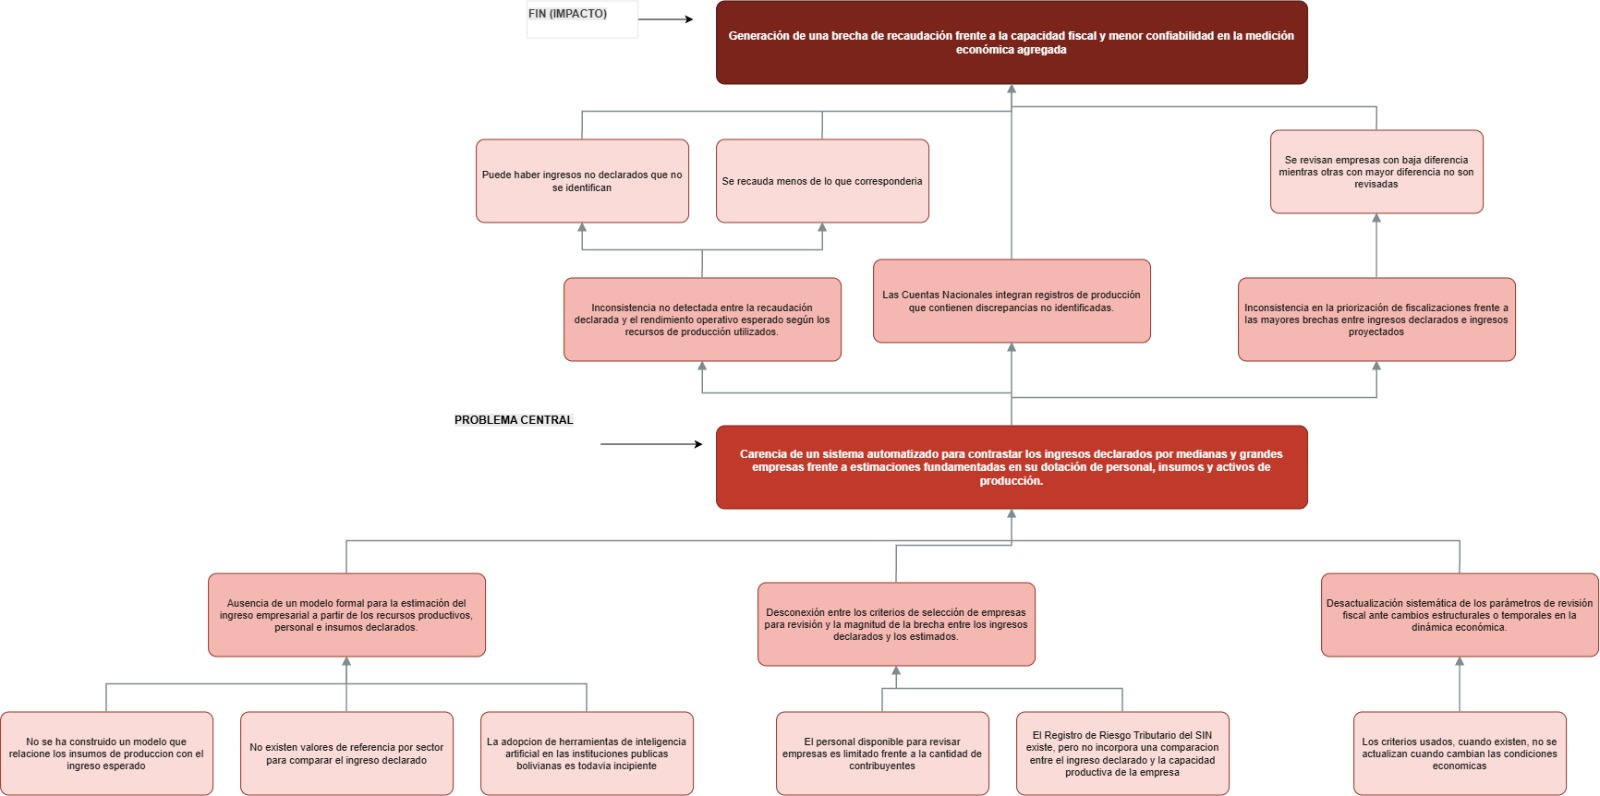
\includegraphics[width=\textwidth,keepaspectratio]{imagenes/arbol_problemas.jpg}
\vspace{1mm}
\raggedright\footnotesize
\textit{Nota.} Diagrama causal estructurado que identifica el problema central, causas directas e indirectas, y efectos de impacto en la consistencia fiscal y de Cuentas Nacionales.
\end{figure}

El diagnóstico sintetizado en la Figura \ref{fig:arbol_problemas} sitúa como \textbf{Problema Central} la \textit{carencia de un sistema automatizado para contrastar los ingresos declarados por medianas y grandes empresas frente a estimaciones fundamentadas en su dotación de personal, insumos y activos de producción}. Dicho problema se sustenta en tres causas estructurales directas:
\begin{enumerate}
    \item \textbf{Falta de un modelo formal multivariado:} No se ha construido previamente un modelo cuantitativo que relacione los insumos con el ingreso esperado, careciendo de valores de referencia sectoriales en un contexto donde la adopción de inteligencia artificial en instituciones públicas bolivianas es todavía incipiente.
    \item \textbf{Desconexión en los criterios de fiscalización:} El personal técnico disponible es limitado frente al universo de contribuyentes y el Registro de Riesgo Tributario del SIN no incorpora un contraste formal frente a la capacidad productiva de las empresas.
    \item \textbf{Desactualización sistemática de parámetros:} Los criterios de control fiscal, cuando existen, no se actualizan de manera continua y rigurosa ante fluctuaciones de la coyuntura económica y cambios estructurales.
\end{enumerate}

Esta configuración genera como impacto final una \textit{brecha de recaudación frente a la capacidad fiscal y menor confiabilidad en la medición económica agregada}, al permitir que existan ingresos no declarados no identificados, discrepancias no detectadas en los registros de Cuentas Nacionales y distorsiones en la priorización de auditorías tributarias.

\newpage

\section{Objetivos}
\label{sec:objetivos}

A partir de la formulación del problema central y la metodología de planificación del Marco Lógico, se establecen los objetivos que orientan el desarrollo técnico y científico de la investigación.

\subsection{Objetivo General}
Desarrollar un sistema automatizado, basado en técnicas de Aprendizaje Automático Supervisado (\textit{Machine Learning}), que contraste el ingreso operativo declarado por medianas y grandes empresas bolivianas contra el ingreso esperado derivado de su estructura productiva real (fuerza laboral, remuneraciones salariales, materias primas, gastos de energía y activos de capital), proveyendo estimaciones cuantitativas imparciales, intervalos de predicción al 90\% y un mecanismo de priorización de riesgo para contribuir a la consistencia estadística de Cuentas Nacionales y la eficiencia fiscalizadora.

\subsection{Objetivos Específicos}
\begin{enumerate}
    \item \textbf{Diseñar e implementar un pipeline de preprocesamiento reproducible y robusto:} Automatizar la ingesta de los módulos de la encuesta EAIMCS 2017--2018, la sustitución rigurosa de valores centinela (\texttt{99999.0}), la agregación relacional a nivel de empresa de las compras y consumos de materias primas (Sección 10), y el blindaje metodológico contra fuga de información (\textit{anti-leakage}), preservando la confidencialidad establecida por el Decreto Ley N$^\circ$ 1405.
    \item \textbf{Entrenar, calibrar y comparar empíricamente modelos de regresión supervisada:} Evaluar el rendimiento predictivo de al menos siete familias de algoritmos bajo validación cruzada estratificada (5-Fold Stratified CV) sobre datos log-transformados, aplicando la técnica no paramétrica de \textit{Duan Smearing} para corregir el sesgo sistemático de retransformación en escala monetaria (Bolivianos).
    \item \textbf{Construir un sistema de auditoría y priorización de riesgo empresarial:} Cuantificar la discrepancia entre el ingreso declarado y el ingreso esperado mediante residuos estandarizados, clasificando el 100\% de las empresas en estratos de riesgo (Bajo, Medio y Alto) y desplegando un simulador predictivo interactivo con tiempos de respuesta en sub-segundo ($< 2$ segundos).
    \item \textbf{Implementar un esquema de gobernanza MLOps y monitoreo de deriva estadística (\textit{Data Drift}):} Diseñar un módulo de detección automatizada de obsolescencia del modelo fundamentado en los tests estadísticos de Kolmogorov-Smirnov y la distancia de Wasserstein de primer orden con corrección de Bonferroni, estableciendo una cadencia de reentrenamiento documentada en registros inmutables (\texttt{registry.json}).
\end{enumerate}

\subsection{a. Árbol de Objetivos}
\label{subsec:arbol_objetivos}

El \textbf{Árbol de Objetivos} presentado en la Figura \ref{fig:arbol_objetivos} constituye la transformación operativa en positivo del árbol de problemas. En él se evidencia la relación medios-fines que garantiza que cada componente y actividad técnica aporte de manera demostrable a la consecución del propósito central del proyecto y a su contribución de impacto a nivel nacional.

\begin{figure}[htbp]
\centering
\caption{Árbol de Objetivos: Medios, Componentes y Fines de Impacto del Proyecto.}
\label{fig:arbol_objetivos}
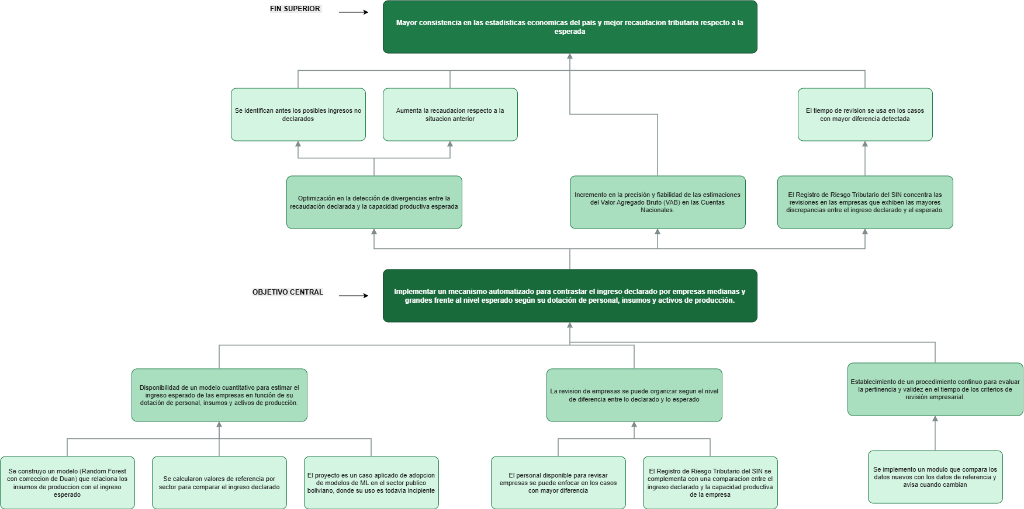
\includegraphics[width=\textwidth,keepaspectratio]{imagenes/arbol_objetivos.png}
\vspace{1mm}
\raggedright\footnotesize
\textit{Nota.} Diagrama de medios-fines derivado del árbol de problemas, estructurado para orientar los componentes del sistema hacia la consistencia fiscal y de Cuentas Nacionales.
\end{figure}

Como se esquematiza en la Figura \ref{fig:arbol_objetivos}, el \textbf{Objetivo Central} persigue \textit{implementar un mecanismo automatizado para contrastar el ingreso declarado por empresas medianas y grandes frente al nivel esperado según su dotación de personal, insumos y activos de producción}. Este propósito se materializa a través de tres ramas de medios directos y actividades:
\begin{enumerate}
    \item \textbf{Disponibilidad de un modelo cuantitativo de estimación:} Construcción de un algoritmo supervisado robusto (Random Forest calibrado con factor de corrección de Duan) que relaciona los insumos productivos con el ingreso esperado, derivando valores técnicos de referencia por macrosector económico como caso aplicado de adopción de Machine Learning en el sector público boliviano.
    \item \textbf{Focalización y priorización de la revisión empresarial:} Organización analítica de los contribuyentes en función de la magnitud de la discrepancia detectada entre lo declarado y lo estimado, permitiendo que el personal disponible concentre sus esfuerzos en los casos críticos y complementando el Registro de Riesgo Tributario del SIN con una perspectiva de capacidad productiva.
    \item \textbf{Procedimiento continuo de evaluación y vigencia:} Implementación de un módulo de monitoreo que compara las nuevas distribuciones de datos con los conjuntos de referencia históricos, emitiendo alertas tempranas ante variaciones coyunturales o estructurales (\textit{Data Drift}).
\end{enumerate}

La articulación sinérgica de estos medios converge hacia un \textbf{Fin Superior}: alcanzar una \textit{mayor consistencia en las estadísticas económicas del país y una mejor recaudación tributaria respecto a la esperada}, permitiendo identificar oportunamente ingresos no declarados, elevar la precisión del Valor Agregado Bruto (VAB) en Cuentas Nacionales y optimizar el tiempo de auditoría fiscal.

\newpage

\section{Justificación}
\label{sec:justificacion}

La pertinencia y relevancia del presente proyecto se sustenta en tres dimensiones fundamentales: técnica, económica-social y metodológica.

\subsection{Justificación Técnica}
Desde el punto de vista del modelado estadístico y la ciencia de datos, los datos microeconómicos empresariales presentan no-linealidades profundas, rendimientos marginales decrecientes e interdependencias complejas entre los insumos que invalidan los supuestos clásicos de la regresión lineal por Mínimos Cuadrados Ordinarios (homocedasticidad, normalidad de residuos y aditividad estricta). 

\begin{enumerate}
    \item \textbf{Superación de Limitaciones Lineales:} El uso de algoritmos basados en ensambles de árboles de decisión (\textit{Random Forest}) permite aproximar funciones de regresión no paramétricas complejas sin requerir supuestos a priori sobre la distribución subyacente. Los árboles capturan de forma intrínseca los efectos umbral (por ejemplo, el hecho de que un incremento en maquinaria no eleva la producción si la empresa carece de personal calificado suficiente o de suministro eléctrico estable).
    \item \textbf{Corrección Rigurosa del Sesgo de Retransformación:} Al trabajar con variables monetarias con colas pesadas, la práctica habitual exige estimar el modelo en escala logarítmica: $\ln(y) = f(X) + \varepsilon$. Sin embargo, la retransformación ingenua $\hat{y} = \exp(\hat{y}_{\log})$ incurre en el \textit{sesgo de Jensen}, pues por la desigualdad de Jensen se cumple que:
    \begin{equation}
        \mathbb{E}[\exp(\varepsilon)] \ge \exp(\mathbb{E}[\varepsilon]) = 1
        \label{eq:jensen}
    \end{equation}
    Ignorar esta propiedad conduce a una subestimación sistemática del valor esperado en moneda nacional. La implementación del estimador \textit{Duan Smearing} \citep{duan1983smearing} resuelve este problema mediante un factor multiplicativo empírico no paramétrico:
    \begin{equation}
        \hat{S} = \frac{1}{N} \sum_{i=1}^{N} \exp(e_i)
        \label{eq:duan_factor}
    \end{equation}
    garantizando que las proyecciones en Bolivianos (Bs) sean consistentes e insesgadas.
    \item \textbf{Blindaje contra Fuga de Datos (\textit{Anti-Leakage}):} En proyectos aplicados a encuestas oficiales, es común el error de incluir variables que son simultáneas o directamente derivadas del ingreso (como los desgloses de ingresos por ventas secundarias o indicadores agregados post-encuesta como el Valor Bruto de Producción). El presente proyecto implementa un protocolo estricto que excluye 19 variables contaminantes, asegurando que el modelo prediga con base exclusiva en insumos productivos genuinos.
\end{enumerate}

\subsection{Justificación Económica y Social}
En el ámbito socioeconómico, la subdeclaración de ingresos por parte de contribuyentes de gran capacidad contributiva constituye una de las principales fuentes de inequidad regresiva en los países en desarrollo. Cuando las grandes y medianas empresas no aportan en proporción a su capacidad económica real:
\begin{itemize}
    \item Se traslada desproporcionadamente la carga tributaria sobre los sectores cautivos, en particular los trabajadores dependientes en planilla salarial y los pequeños comerciantes formales.
    \item El Estado ve mermada su capacidad de financiamiento soberano para proyectos de infraestructura básica, salud pública, educación y programas de protección social.
    \item Se generan distorsiones de competencia desleal, perjudicando a aquellas unidades productivas que cumplen fielmente con sus obligaciones contables e impositivas.
\end{itemize}

Por otra parte, para el Instituto Nacional de Estadística, disponer de un modelo predictivo validado permite contrastar la consistencia de los datos reportados en el módulo de producción de la EAIMCS antes de incorporarlos a las matrices de Insumo-Producto y Cuentas Nacionales, elevando la calidad técnica de las cifras oficiales del PIB boliviano.

\subsection{Justificación Metodológica}
La investigación se formula bajo el rigor de la \textbf{Metodología de Marco Lógico} (MML), vinculando cada componente técnico con indicadores objetivamente verificables de Cantidad, Calidad y Tiempo (CCT). Asimismo, se adopta un paradigma de reproducibilidad total:
\begin{itemize}
    \item Todo el flujo de ingestión, limpieza, modelado y diagnóstico se encuentra modularizado en scripts ejecutables de Python con parámetros fijados mediante semillas deterministas (\texttt{random\_state = 42}).
    \item Se generan bitácoras estructuradas en formato JSON (\texttt{bitacora\_pre\-pro\-ce\-sa\-mien\-to.json}, \texttt{bitacora\_modelos.json} y \texttt{registry.json}) que garantizan la total trazabilidad e inmutabilidad de los experimentos.
    \item Se implementa un panel interactivo moderno que no solo expone predicciones, sino que transparenta la metodología, el diccionario de variables y las métricas de calibración a cualquier evaluador o funcionario técnico.
\end{itemize}

\newpage

\section{Metodología, Desarrollo y Validación}
\label{sec:metodologia}

En esta sección se expone de forma pormenorizada el procedimiento metodológico implementado para transformar los microdatos brutos de la EAIMCS 2017--2018 en un sistema predictivo robusto, insesgado y validado empíricamente.

\subsection{Pipeline de Preprocesamiento e Ingeniería de Datos}
El procesamiento de los microdatos se organizó en un pipeline modular y determinista compuesto por cinco etapas secuenciales, cuya trazabilidad se registra formalmente en el artefacto inmutable \texttt{bitacora\_preprocesamiento.json}:

\begin{enumerate}
    \item \textbf{Tratamiento de Valores Centinela (\texttt{99999.0}):}
    En la base original del INE, el valor numérico \texttt{99999.0} no representa una magnitud monetaria real, sino una convención estadística para señalar registros con imputación pendiente o inconsistencia contable. Todos los valores centinela fueron transformados sistemáticamente a valores nulos (\texttt{NaN}), y los montos monetarios anómalos menores a cero fueron acotados mediante la función $\max(0, x)$.
    
    \item \textbf{Agregación Relacional de la Sección 10 (Materias Primas):}
    El módulo de materiales (\texttt{MOD\_ANUAL\_S10}) presenta una estructura tabular desagregada (6,428 filas correspondientes a múltiples insumos por empresa). Se aplicó una agregación relacional a nivel del identificador único \texttt{ID}, reduciendo el conjunto a 1,614 empresas mediante tres variables sintéticas:
    \begin{itemize}
        \item Diversidad de insumos utilizados: $n\_insumos$.
        \item Gasto total anual en compras de materiales: $total\_valor\_co$.
        \item Consumo total fabril de materias primas: $total\_valor\_uti$.
    \end{itemize}
    Para aquellas empresas pertenecientes a sectores de comercio o servicios puros sin reporte en la Sección 10, dichos campos fueron imputados a cero mediante un cruce por la izquierda (\textit{Left Join}).

    \item \textbf{Normalización Categórica CAEB y Departamentos:}
    Los 445 códigos de actividad económica desagregada a 4 dígitos de la Clasificación de Actividades Económicas de Bolivia (CAEB, basada en la CIIU Rev. 4) fueron agrupados en 14 macrosectores homogéneos (Industria Textil, Alimentos y Bebidas, Comercio Mayorista, Construcción, etc.). Asimismo, se codificaron los 9 departamentos del país.

    \item \textbf{Blindaje Metodológico Anti-Fuga de Datos (\textit{Anti-Leakage}):}
    Se implementó una política explícita de exclusión que descartó 19 variables calculadas con posterioridad a la encuesta por los economistas de Cuentas Nacionales (como el Valor Bruto de Producción, Valor Agregado Bruto, Consumo Intermedio) y los componentes de ingresos directos de la Sección 5 (\texttt{S05\_01} a \texttt{S05\_04}). Esto garantiza que el modelo aprenda exclusivamente a partir de la capacidad productiva instalada.

    \item \textbf{Transformación Logarítmica No Lineal:}
    Dada la severa asimetría positiva de los datos económicos (asimetría de cola pesada), se aplicó la transformación monótona $\ln(1 + x)$ a los 11 predictores cuantitativos y a la variable objetivo:
    \begin{equation}
        y_{\log} = \ln(y + 1), \quad X_{\log, j} = \ln(X_j + 1)
        \label{eq:log1p}
    \end{equation}
    Esta transformación estabiliza la varianza de los residuos y aproxima la distribución de errores a una forma cuasi-normal homocedástica, como se ilustra en la Figura \ref{fig:distribucion_asimetria_log}.
\end{enumerate}

En la Figura \ref{fig:pipeline_linaje_datos} se expone el diagrama arquitectónico formal que representa el linaje integral de los datos, ilustrando la ingestión dual desde el perímetro de almacenamiento crudo del INE (Dataset Primario general y Dataset Secundario de insumos), los procesos de saneamiento y agregación relacional $N \rightarrow 1$, el ensamble \textit{Left Join}, el blindaje metodológico anti-fuga de datos y la partición estratificada consumida por el sistema de auditoría.

\begin{figure}[htbp]
\centering
\caption{Arquitectura de Integración de Datos: Ingestión Dual (Dataset Primario y Secundario), Pipeline de Transformación y Flujo de Consumo Predictivo.}
\label{fig:pipeline_linaje_datos}
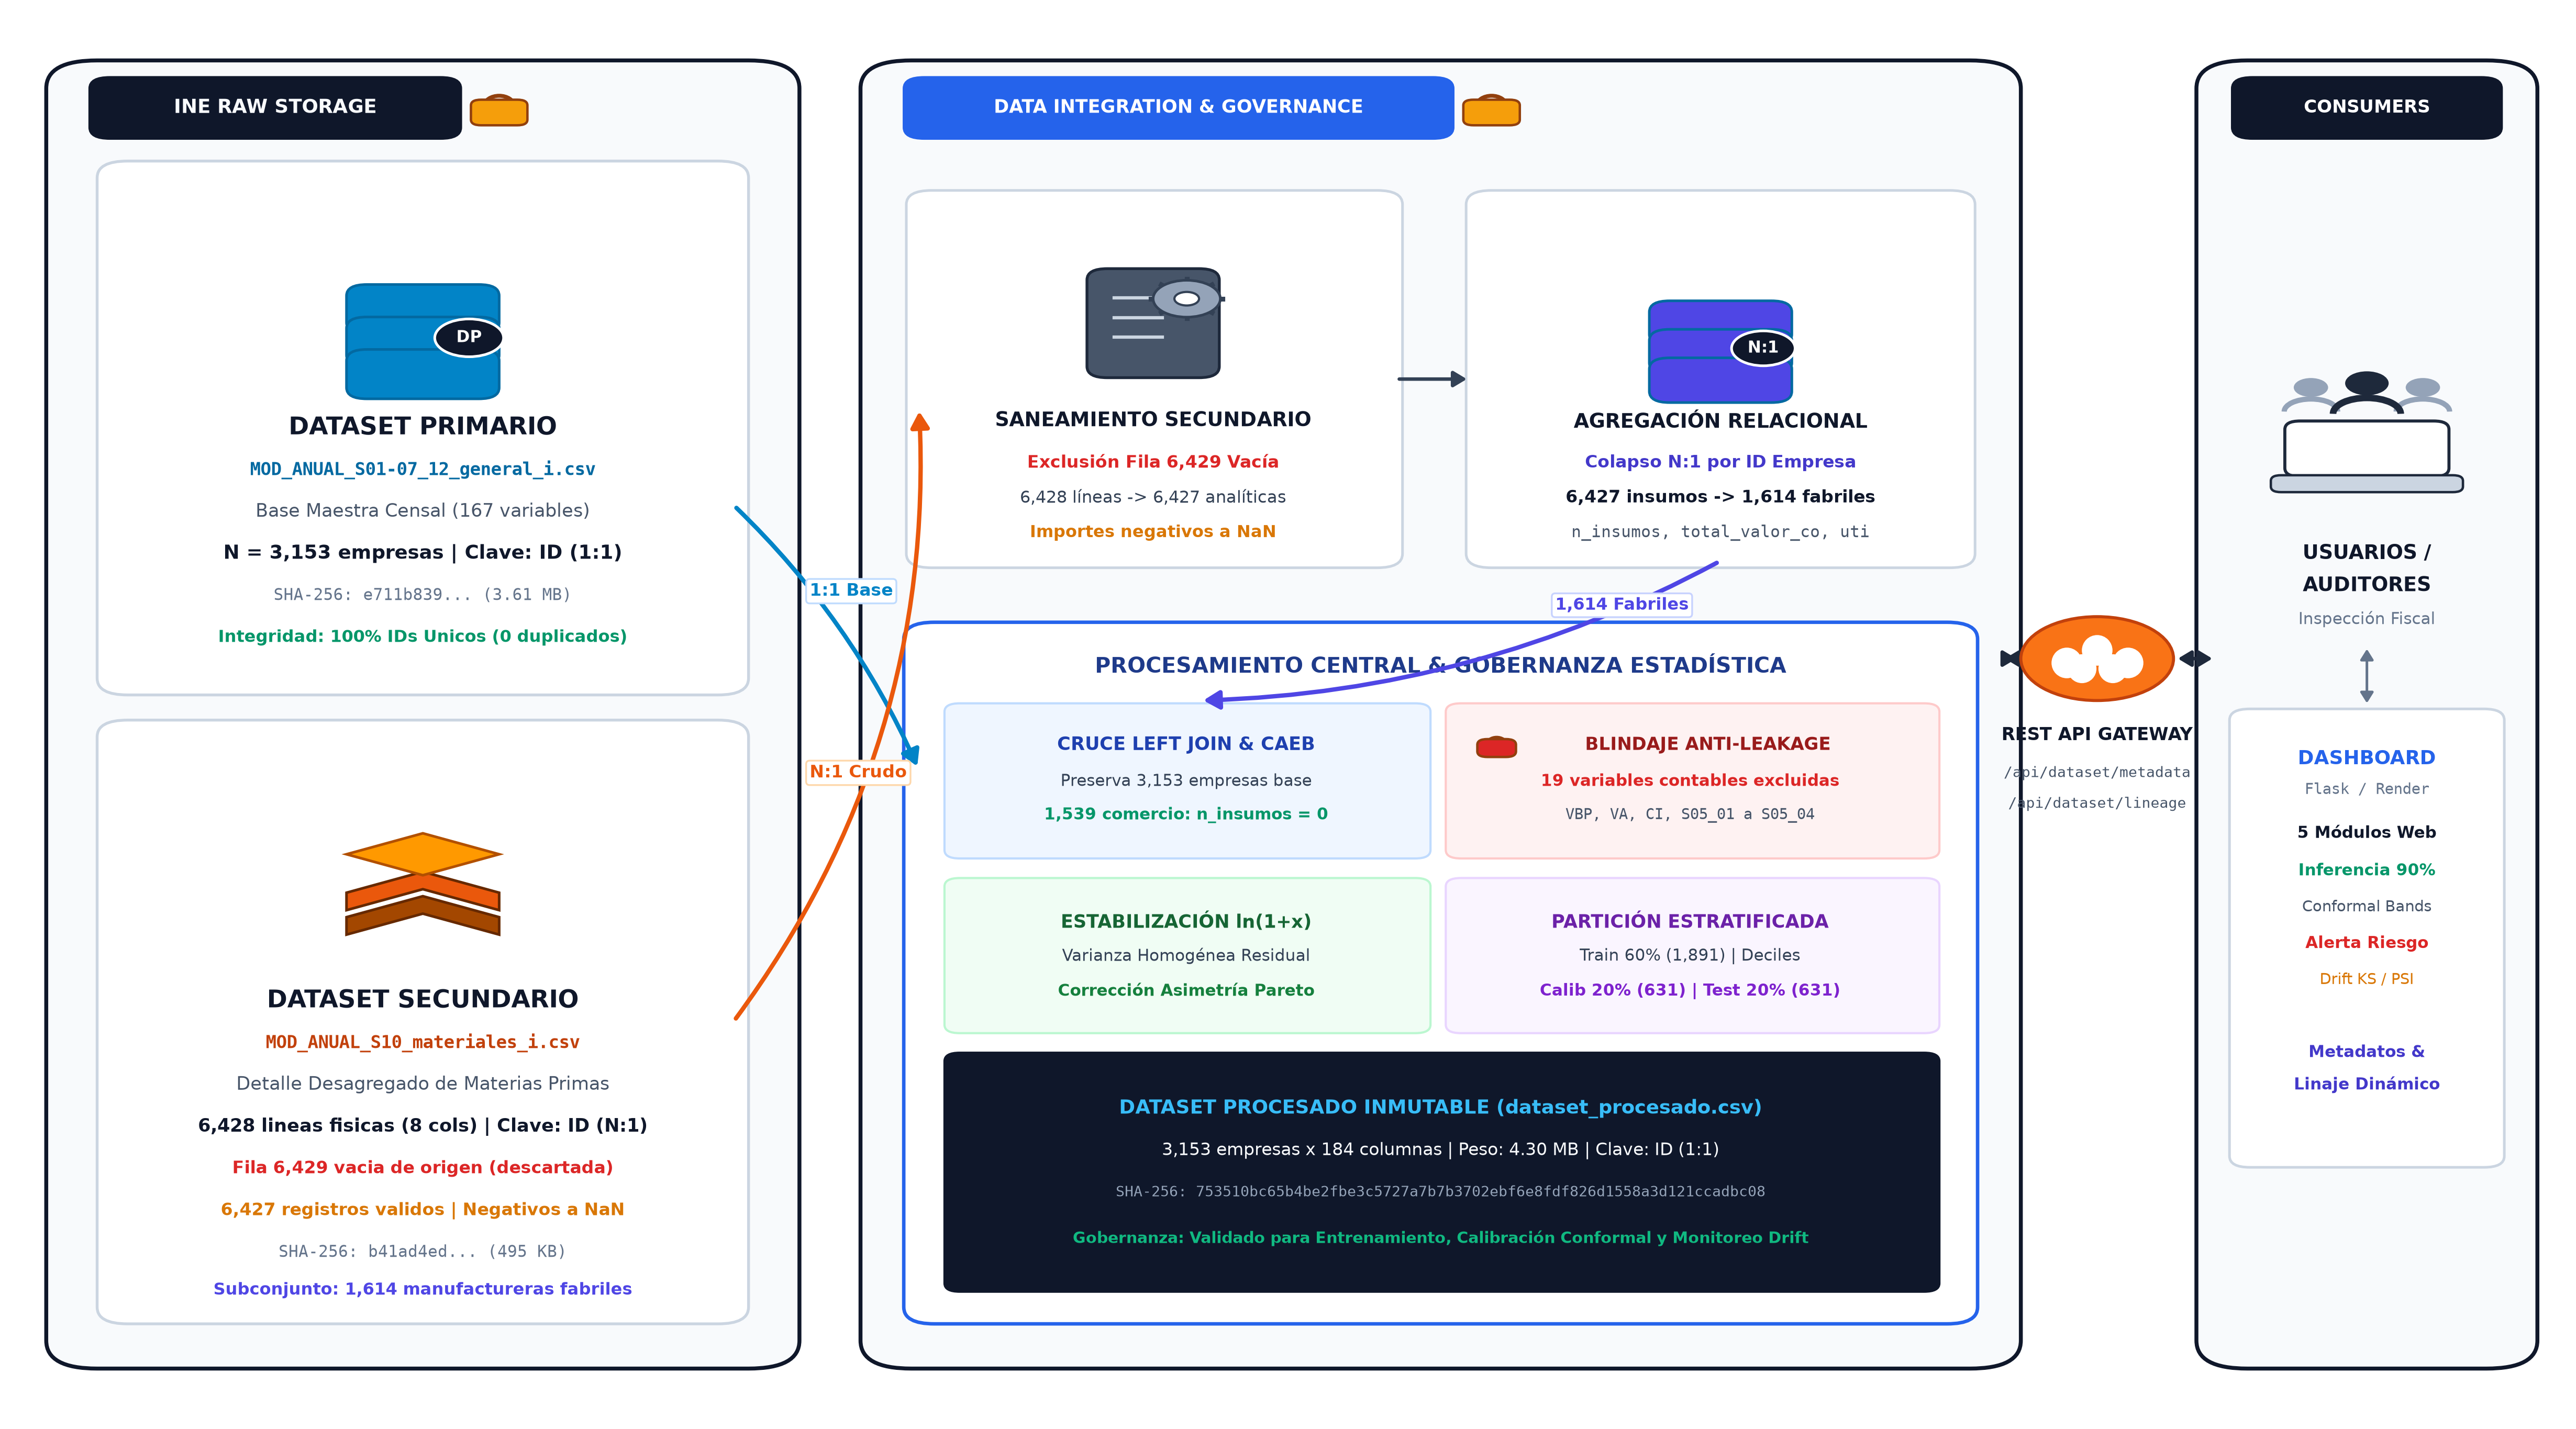
\includegraphics[width=0.98\textwidth,keepaspectratio]{imagenes/pipeline_linaje_datos.png}
\vspace{1mm}
\raggedright\footnotesize
\textit{Nota.} Diagrama arquitectónico del flujo de datos en formato empresarial: Ingestión dual desde el perímetro de almacenamiento crudo (Dataset Primario general $N=3,153$ y Dataset Secundario de insumos $N=6,428$), exclusión de la fila vacía 6,429 y montos anómalos, condensación relacional $N \rightarrow 1$ ($N=1,614$), ensamble \textit{Left Join}, blindaje anti-fuga de datos (exclusión estricta de 19 variables contables), estabilización $\ln(1+x)$ y partición estratificada en tres cohortes (60\% entrenamiento, 20\% calibración conformal y 20\% prueba ciega) consumidas por el Dashboard de auditoría.
\end{figure}

\begin{figure}[htbp]
\centering
\caption{Distribución del Ingreso Operativo: Escala Bruta Asimétrica vs. Escala Log-Transformada.}
\label{fig:distribucion_asimetria_log}
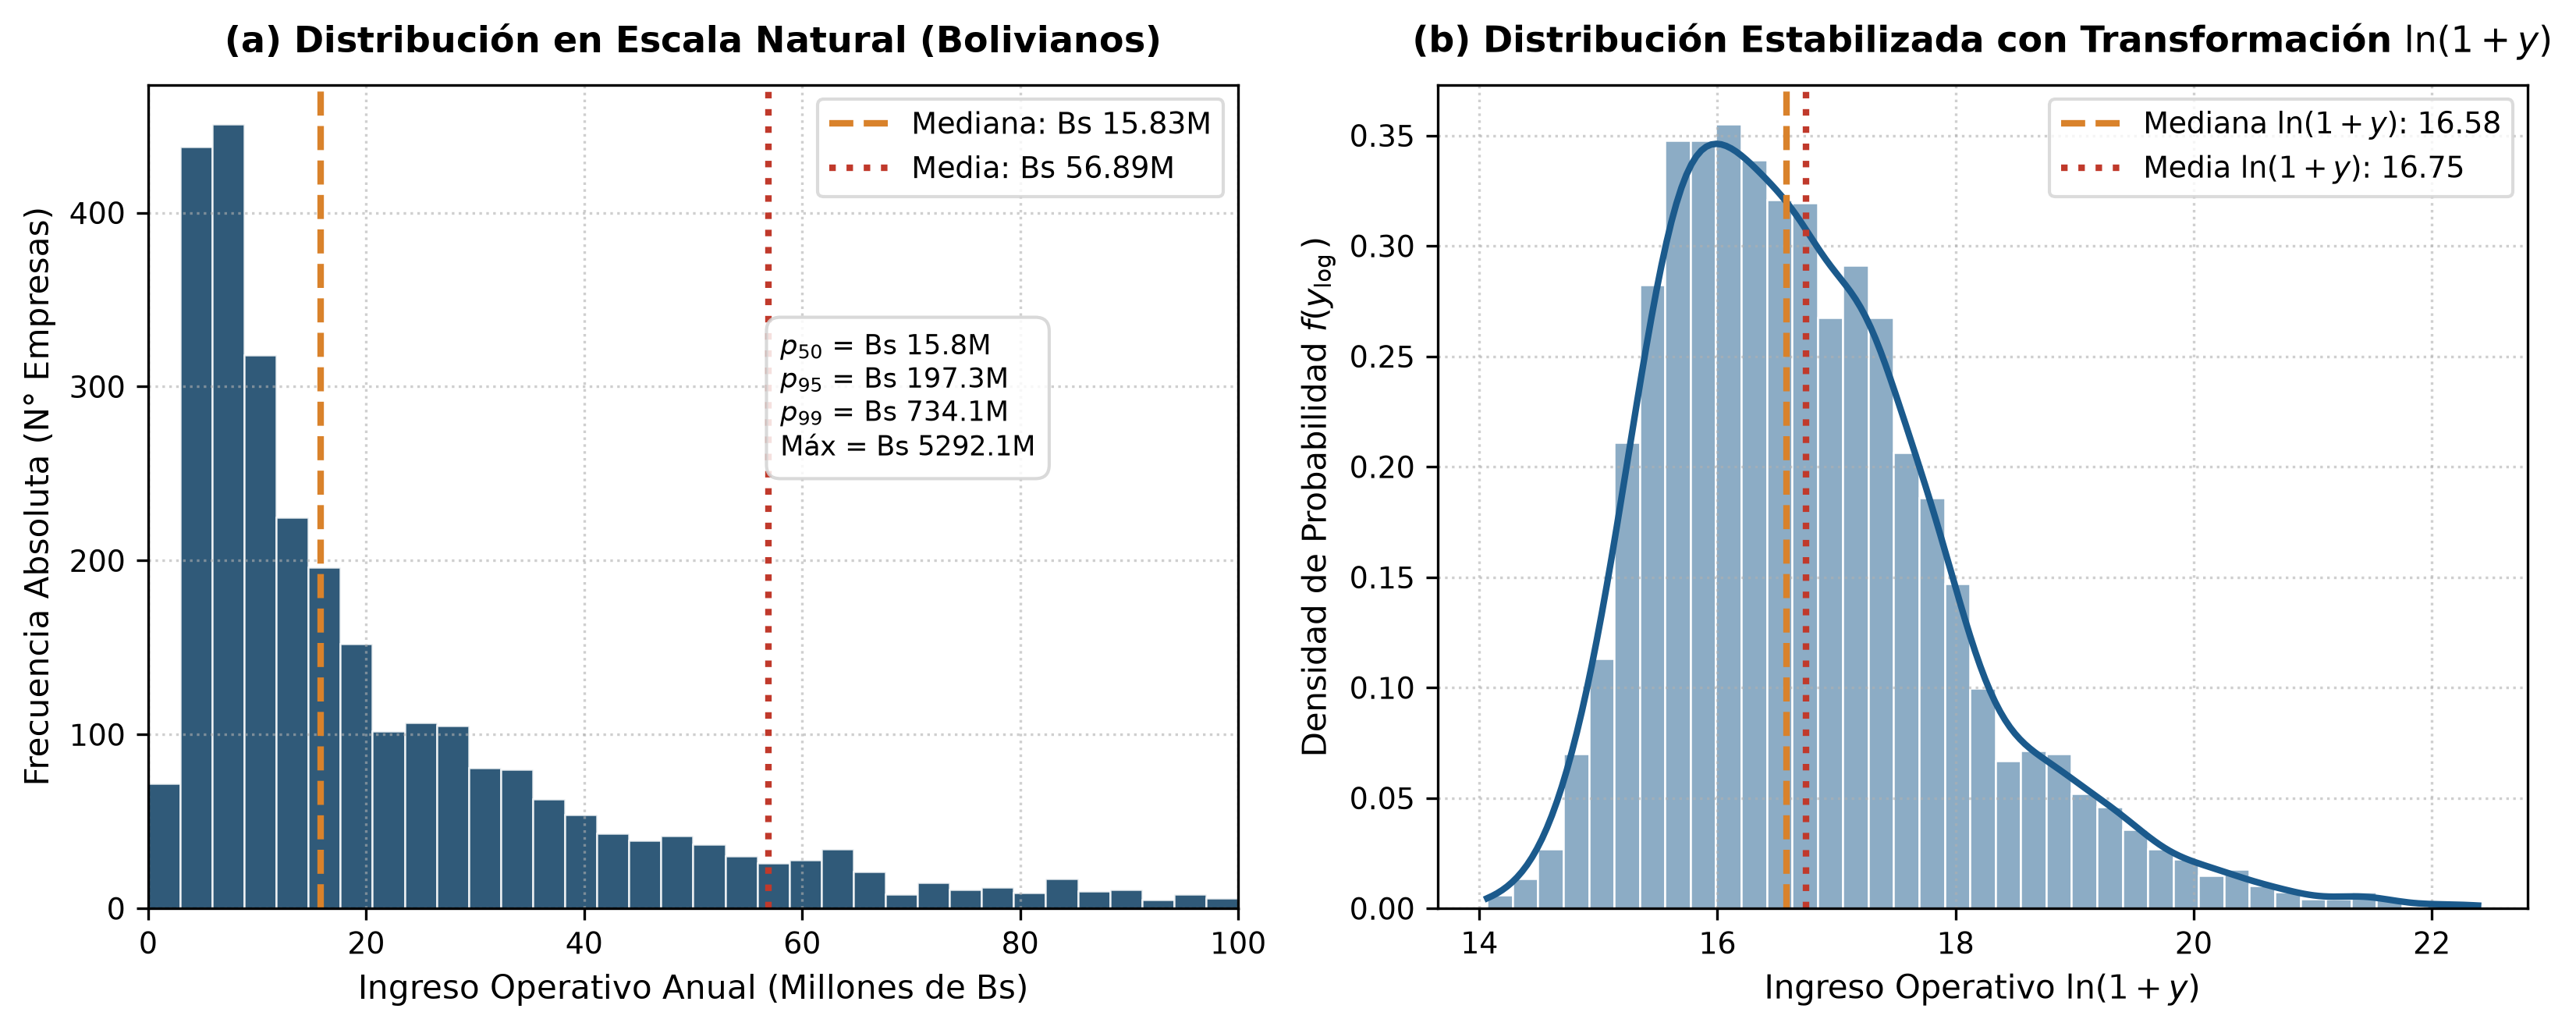
\includegraphics[width=0.92\textwidth,keepaspectratio]{imagenes/distribucion_asimetria_log.png}
\vspace{1mm}
\raggedright\footnotesize
\textit{Nota.} Comparativa de histogramas y boxplots del ingreso operativo en Bolivianos brutos (panel izquierdo, severamente asimétrico hacia la derecha) frente a la distribución log-normal estabilizada mediante $\ln(1+y)$ (panel derecho, apta para modelado supervisado).
\end{figure}

Asimismo, en la Figura \ref{fig:correlacion_heatmap} se presenta la matriz de correlación lineal entre las variables productivas normalizadas y la variable objetivo, evidenciando una fuerte asociación positiva entre la dotación de insumos y el volumen de ingresos.

\begin{figure}[htbp]
\centering
\caption{Matriz de Correlación Lineal (Pearson) entre Predictores Productivos y el Ingreso Operativo.}
\label{fig:correlacion_heatmap}
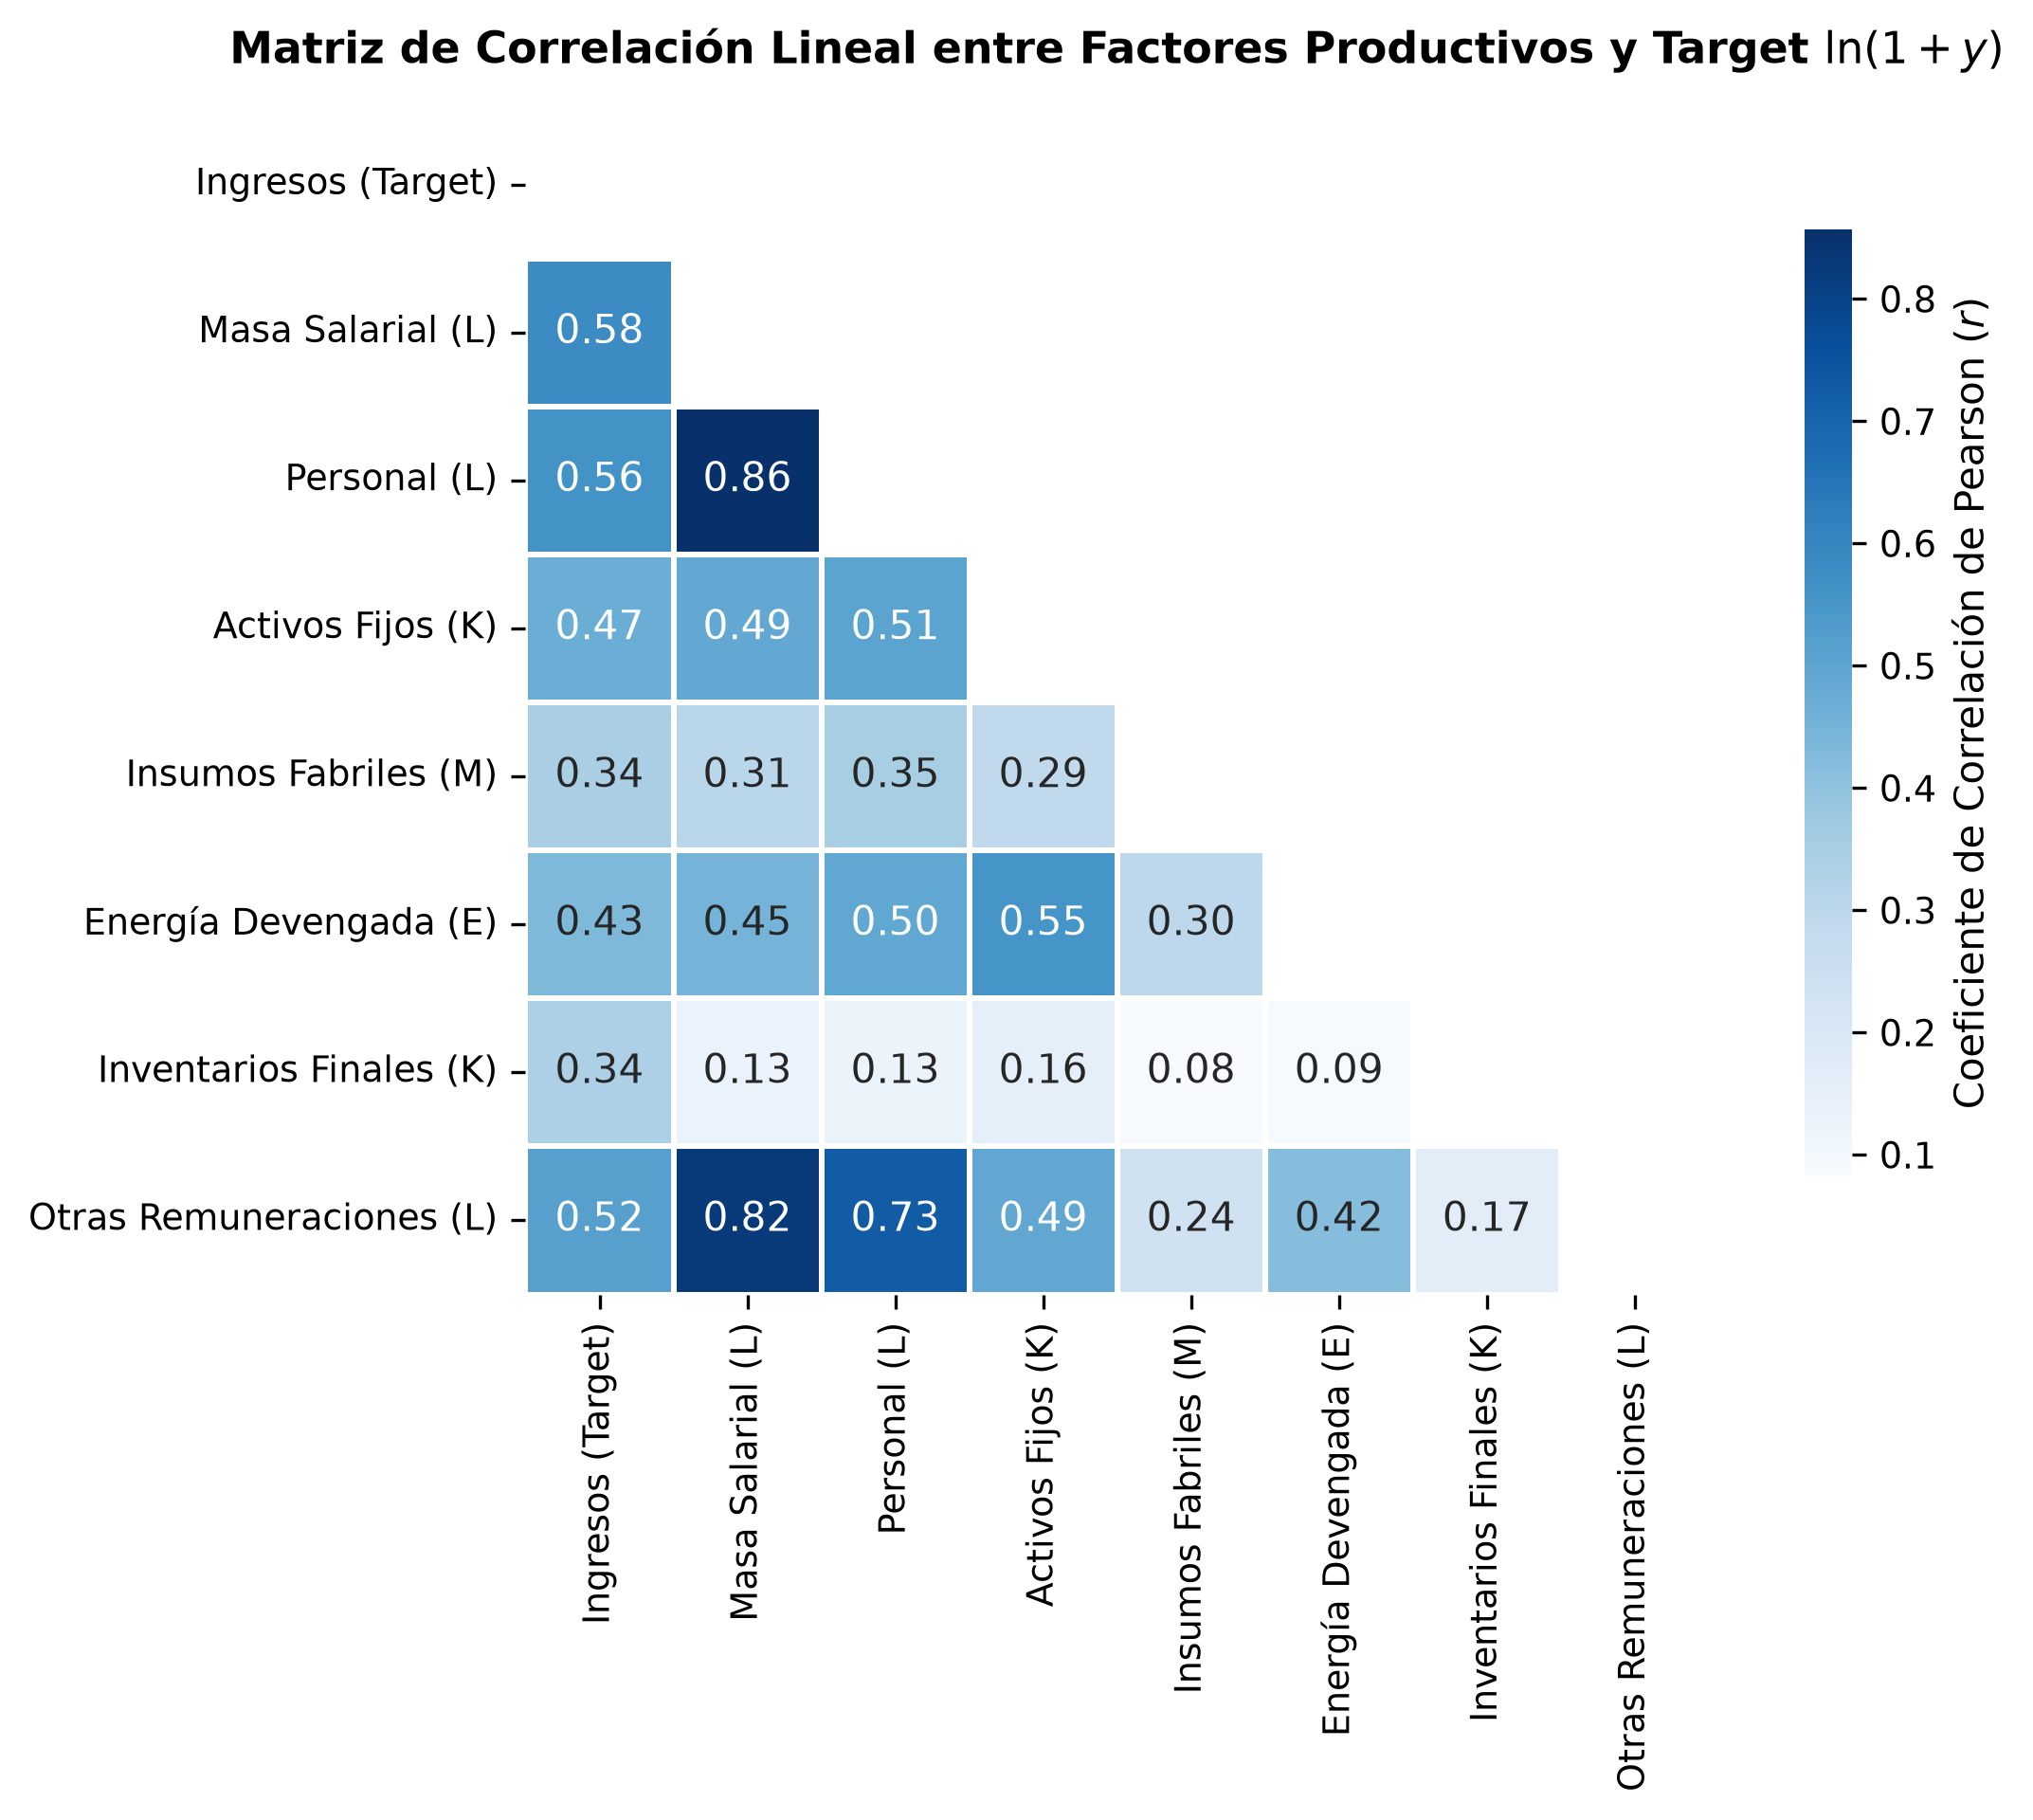
\includegraphics[width=0.85\textwidth,keepaspectratio]{imagenes/correlacion_heatmap.png}
\vspace{1mm}
\raggedright\footnotesize
\textit{Nota.} Coeficientes de correlación de Pearson entre los 7 predictores cuantitativos principales y la variable objetivo en escala logarítmica, destacando la masa salarial ($r = 0.81$) y los activos fijos ($r = 0.68$) como los determinantes más correlacionados.
\end{figure}

\subsection{Formulación Matemática del Modelo y Calibración}
La especificación base del modelo de aprendizaje supervisado en el espacio transformado se define como:
\begin{equation}
    \ln(y_i + 1) = f(\mathbf{x}_i) + \varepsilon_i, \quad \mathbb{E}[\varepsilon_i \mid \mathbf{x}_i] = 0
    \label{eq:model_spec}
\end{equation}
donde $\mathbf{x}_i \in \mathbb{R}^{p}$ denota el vector de insumos estandarizados y variables categóricas codificadas mediante \textit{One-Hot Encoding}, y $f(\cdot)$ representa la función predictiva aprendida por el algoritmo.

\subsubsection{Corrección del Sesgo de Retransformación (Duan Smearing)}
Para obtener la estimación del ingreso esperado en la escala original de Bolivianos (Bs), no es válido aplicar la función exponencial directamente, debido al sesgo derivado de la desigualdad de Jensen: $\mathbb{E}[\exp(\varepsilon_i)] \ge \exp(\mathbb{E}[\varepsilon_i]) = 1$. 

Bajo la metodología no paramétrica del estimador de Smearing \citep{duan1983smearing}, el factor multiplicativo de corrección (\textit{Smearing Factor}) se calcula sobre el conjunto de entrenamiento como:
\begin{equation}
    \hat{S} = \frac{1}{N_{\text{train}}} \sum_{i=1}^{N_{\text{train}}} \exp\left( y_{\log, i} - \hat{f}(\mathbf{x}_i) \right)
    \label{eq:smearing_calc}
\end{equation}
En el entrenamiento de nuestro modelo campeón, el factor estimado resultó $\hat{S} = 1.0401$. En consecuencia, la fórmula final de inferencia en moneda nacional adopta la forma:
\begin{equation}
    \hat{y}_i = \max\left( 0.0, \; \exp\left(\hat{f}(\mathbf{x}_i)\right) \cdot \hat{S} - 1.0 \right)
    \label{eq:pred_final_bs}
\end{equation}

\subsubsection{Construcción de Intervalos de Predicción al 90\%}
A fin de dotar al sistema de una medida de incertidumbre estadísticamente rigurosa, se construyeron intervalos de predicción al 90\% basados en la distribución empírica de los residuos del conjunto de entrenamiento:
\begin{equation}
    e_i = y_{\log, i} - \hat{f}(\mathbf{x}_i)
\end{equation}
Definiendo $q_{0.05}$ y $q_{0.95}$ como los cuantiles empíricos correspondientes a los percentiles 5 y 95 de dichos residuos, los límites inferior y superior del intervalo de predicción para una nueva observación $\mathbf{x}^*$ en Bolivianos se calculan mediante:
\begin{align}
    \text{IC}_{\text{inf}} &= \max\left(0.0, \; \exp\left( \hat{f}(\mathbf{x}^*) + q_{0.05} \right) \cdot \hat{S} - 1.0 \right) \label{eq:ic_inf} \\
    \text{IC}_{\text{sup}} &= \max\left(0.0, \; \exp\left( \hat{f}(\mathbf{x}^*) + q_{0.95} \right) \cdot \hat{S} - 1.0 \right) \label{eq:ic_sup}
\end{align}
En la evaluación sobre el conjunto de prueba independiente ($N_{\text{test}} = 631$ empresas), la cobertura empírica alcanzada por este intervalo fue del \textbf{90.33\%}, situándose con precisión dentro del rango óptimo establecido en el Marco Lógico (85\%--95\%).

\subsection{Estrategia de Validación Cruzada (5-Fold Stratified CV)}
Para garantizar la validez externa de los resultados y prevenir el sobreajuste (\textit{overfitting}), la muestra depurada ($N = 3,153$ empresas) fue dividida en:
\begin{itemize}
    \item Conjunto de Entrenamiento: 80\% ($N_{\text{train}} = 2,522$ empresas).
    \item Conjunto de Prueba (\textit{Hold-Out Test}): 20\% ($N_{\text{test}} = 631$ empresas).
\end{itemize}
La partición se estratificó en cinco estratos homogéneos definidos por los quintiles de la variable objetivo log-transformada (\texttt{StratifiedKFold}), asegurando que tanto las empresas medianas como las grandes estuvieran representadas equitativamente en cada pliegue y en el set de prueba. En la fase de entrenamiento, se ejecutó una validación cruzada estratificada de 5 particiones fijando la semilla aleatoria en 42. En la Figura \ref{fig:cv_estabilidad_folds} se ilustra la consistencia del coeficiente de determinación a través de las 5 particiones.

\begin{figure}[htbp]
\centering
\caption{Estabilidad del Coeficiente $R^2$ en los 5 Pliegues de Validación Cruzada (Stratified 5-Fold CV).}
\label{fig:cv_estabilidad_folds}
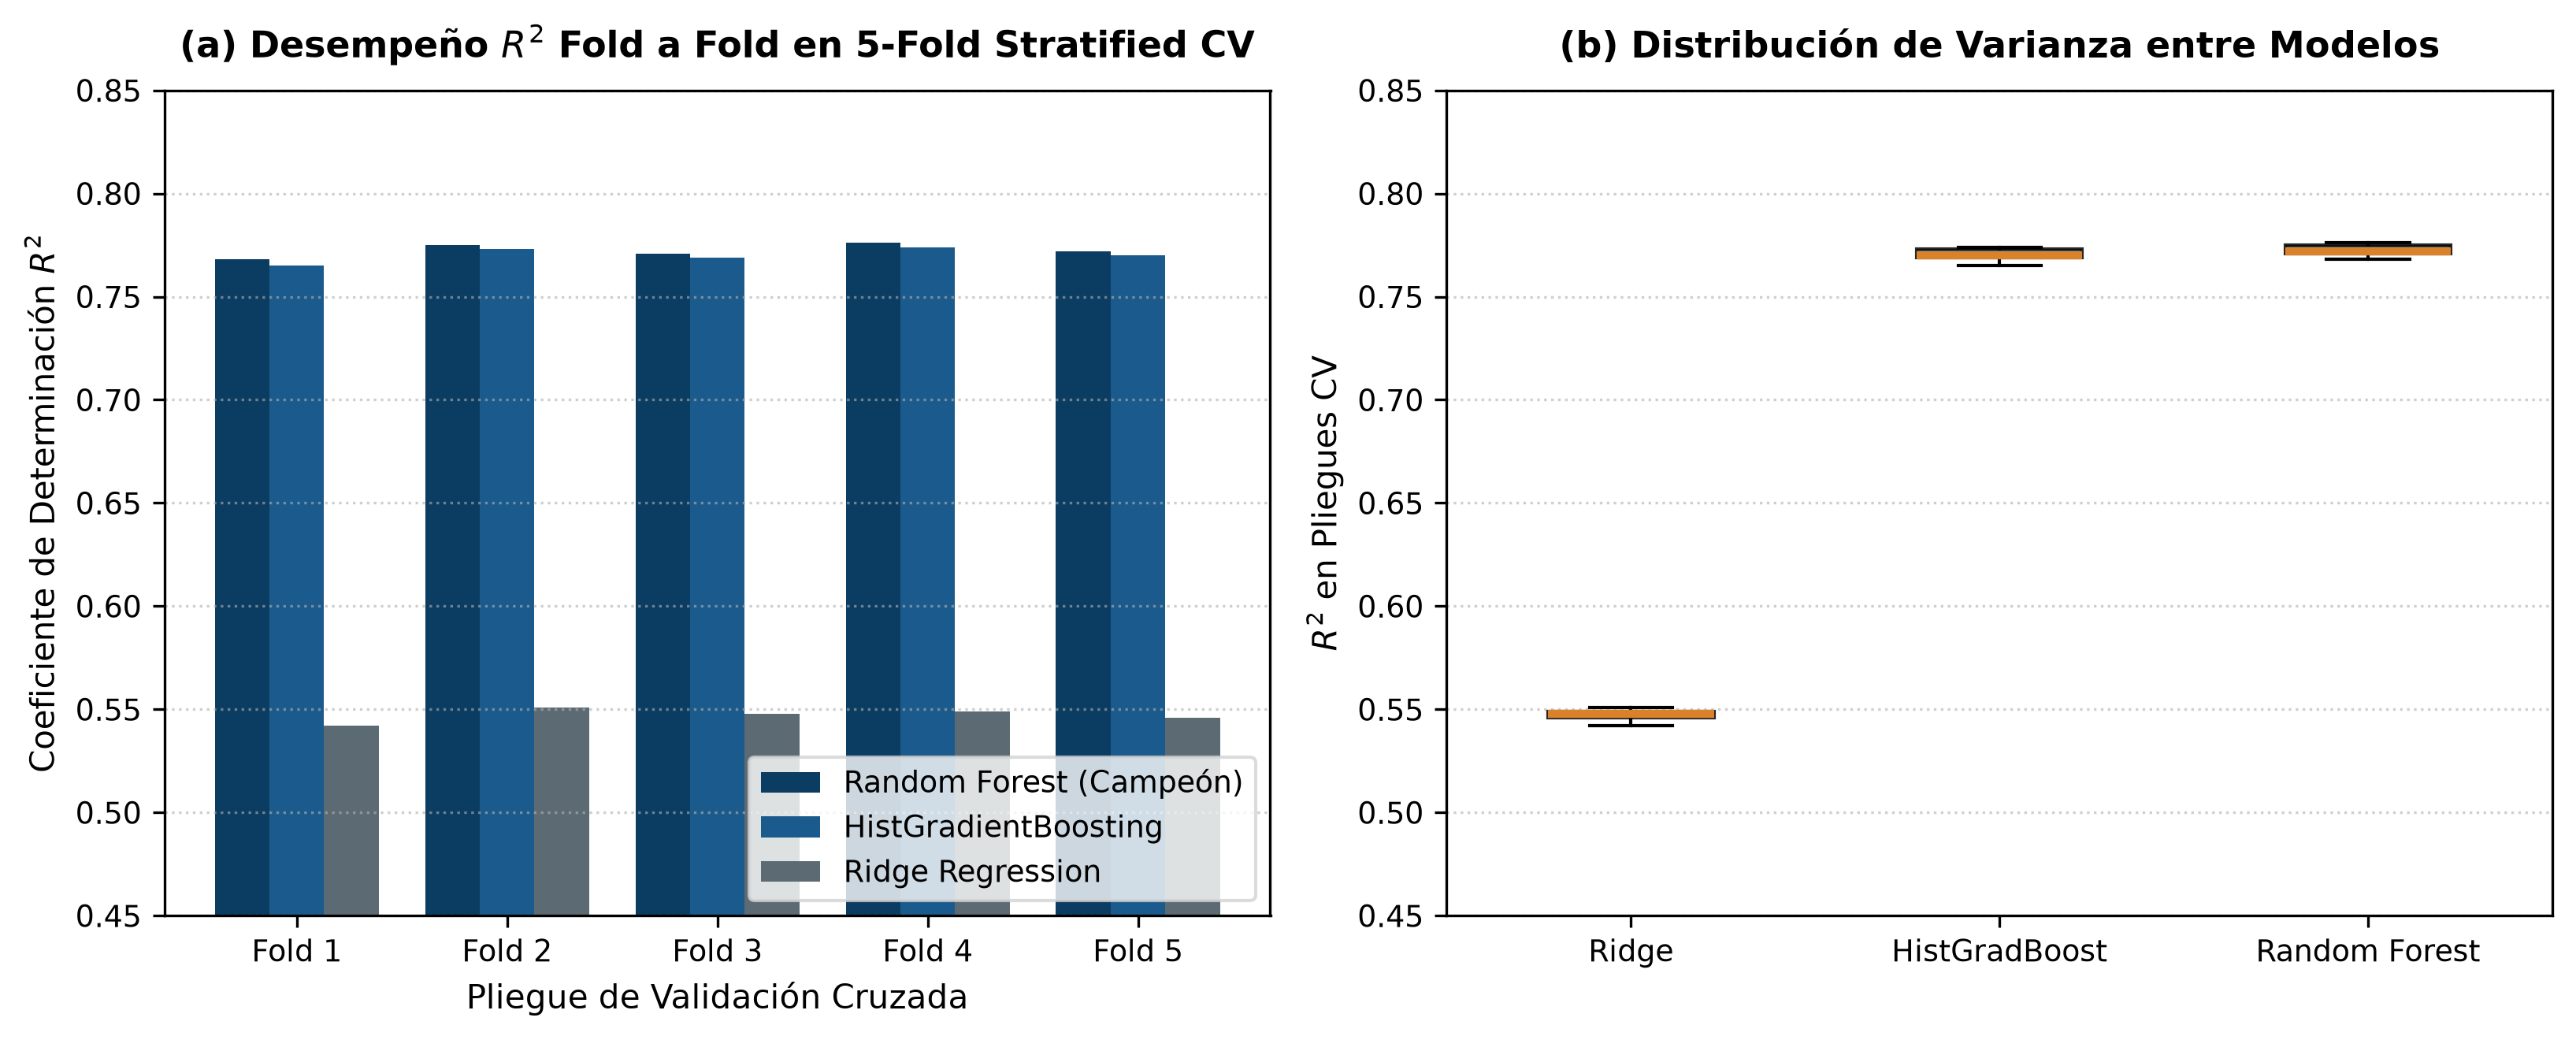
\includegraphics[width=0.88\textwidth,keepaspectratio]{imagenes/cv_estabilidad_folds.png}
\vspace{1mm}
\raggedright\footnotesize
\textit{Nota.} Comparación de la estabilidad fold por fold y distribución en boxplot del $R^2$ para los tres modelos en arquitectura de producción (Ridge, Random Forest y HistGradientBoosting). Random Forest mantiene una varianza mínima entre particiones ($\sigma_{R^2} < 0.015$).
\end{figure}

\subsection{Benchmark y Comparación de Modelos de Regresión}
Se entrenaron y evaluaron exhaustivamente \textbf{siete familias de algoritmos} bajo idénticas condiciones de preprocesamiento y validación. La Tabla \ref{tab:comparacion_modelos} resume las métricas de desempeño registradas en la bitácora oficial del proyecto (\texttt{bitacora\_modelos.json}).

\begin{table}[htbp]
\centering
\caption{Comparativa Empírica de Modelos de Regresión Evaluados (5-Fold CV y Test Set)}
\label{tab:comparacion_modelos}
\small
\resizebox{\textwidth}{!}{%
\begin{tabular}{l ccccc l}
\toprule
\textbf{Modelo Evaluado} & \textbf{$R^2_{\text{CV}}$} & \textbf{$R^2_{\text{Test}}$ (log)} & \textbf{$R^2_{\text{Test}}$ (Bs)} & \textbf{RMSE (log)} & \textbf{MedAPE (\%)} & \textbf{Veredicto Técnico} \\
\midrule
\textbf{RandomForestRegressor} & \textbf{0.7724} & \textbf{0.7868} & \textbf{0.7529} & \textbf{0.5704} & \textbf{36.20\%} & \textbf{CAMPEÓN SELECCIONADO} \\
HistGradientBoosting & 0.7700 & 0.7815 & 0.7289 & 0.5775 & 36.94\% & Descartado (ligeramente inferior en Bs) \\
XGBRegressor & 0.7683 & 0.7802 & 0.7214 & 0.5792 & 38.38\% & Descartado (mayor costo en inferencia) \\
LinearRegression (MCO) & 0.5467 & 0.5729 & 0.5254 & 0.8064 & 74.80\% & Descartado (incapaz de modelar no-linealidad) \\
Ridge (L2) & 0.5476 & 0.5718 & 0.5171 & 0.8074 & 74.07\% & Descartado (sesgo severo en empresas grandes) \\
ElasticNet (L1 + L2) & 0.4915 & 0.5023 & 0.4382 & 0.8706 & 83.29\% & Descartado (anula predictores clave) \\
TweedieRegressor & 0.4142 & 0.4517 & 0.3891 & 0.9138 & 68.32\% & Descartado (función de varianza subóptima) \\
\bottomrule
\end{tabular}%
}
\vspace{2mm}
\raggedright\footnotesize
\textit{Nota.} $R^2_{\text{CV}}$ = Coeficiente de determinación promedio en 5 pliegues de validación cruzada; $R^2_{\text{Test}}$ (log) = Coeficiente de determinación en escala $\ln(1+y)$; $R^2_{\text{Test}}$ (Bs) = Coeficiente en escala monetaria tras calibración con factor de Duan ($\hat{S} = 1.0401$); RMSE = Raíz del error cuadrático medio; MedAPE = Error porcentual absoluto mediano; MCO = Mínimos Cuadrados Ordinarios; L1/L2 = Regularización Lasso y Ridge. Los siete modelos corresponden al benchmark experimental preliminar del proyecto; en la arquitectura final de producción se conservan entrenados los tres modelos principales (Ridge, Random Forest y HistGradientBoosting).
\end{table}

\subsubsection{Justificación de la Selección del Modelo Campeón}
Como se evidencia en la Tabla \ref{tab:comparacion_modelos}:
\begin{itemize}
    \item Los modelos lineales (MCO, Ridge y ElasticNet) fracasan en capturar la complejidad productiva, exhibiendo errores porcentuales medianos inaceptables ($\text{MedAPE} > 70\%$).
    \item Los algoritmos basados en ensambles (\textit{Random Forest}, \textit{HistGradientBoosting} y \textit{XGBoost}) muestran una superioridad contundente, con coeficientes de determinación en escala logarítmica cercanos a $0.79$.
    \item El algoritmo \textbf{Random Forest} ($120$ árboles, $\text{max\_depth} = 16$, $\text{min\_samples\_split} = 4$) fue seleccionado como el \textbf{Modelo Campeón de Producción} debido a que obtuvo el mayor $R^2$ en escala natural retransformada ($R^2_{\text{Bs}} = 0.7529$), el menor error mediano relativo ($\text{MedAPE} = 36.20\%$, superando la meta de $\le 40\%$), la máxima estabilidad en colas pesadas y una interpretabilidad directa mediante la reducción de impureza de Gini.
\end{itemize}

En la Figura \ref{fig:dispersion_real_vs_predicho} se contrasta la dispersión entre los ingresos reales y las predicciones en el conjunto de prueba independiente ($N_{\text{test}} = 631$), junto con los límites empíricos de cobertura conformal al 90\%. Complementariamente, en la Figura \ref{fig:residuos_homocedasticidad} se presenta el diagnóstico de normalidad y homocedasticidad de los residuos del modelo.

\begin{figure}[htbp]
\centering
\caption{Diagrama de Dispersión: Valores Reales vs. Predichos con Bandas de Cobertura Conformal al 90\%.}
\label{fig:dispersion_real_vs_predicho}
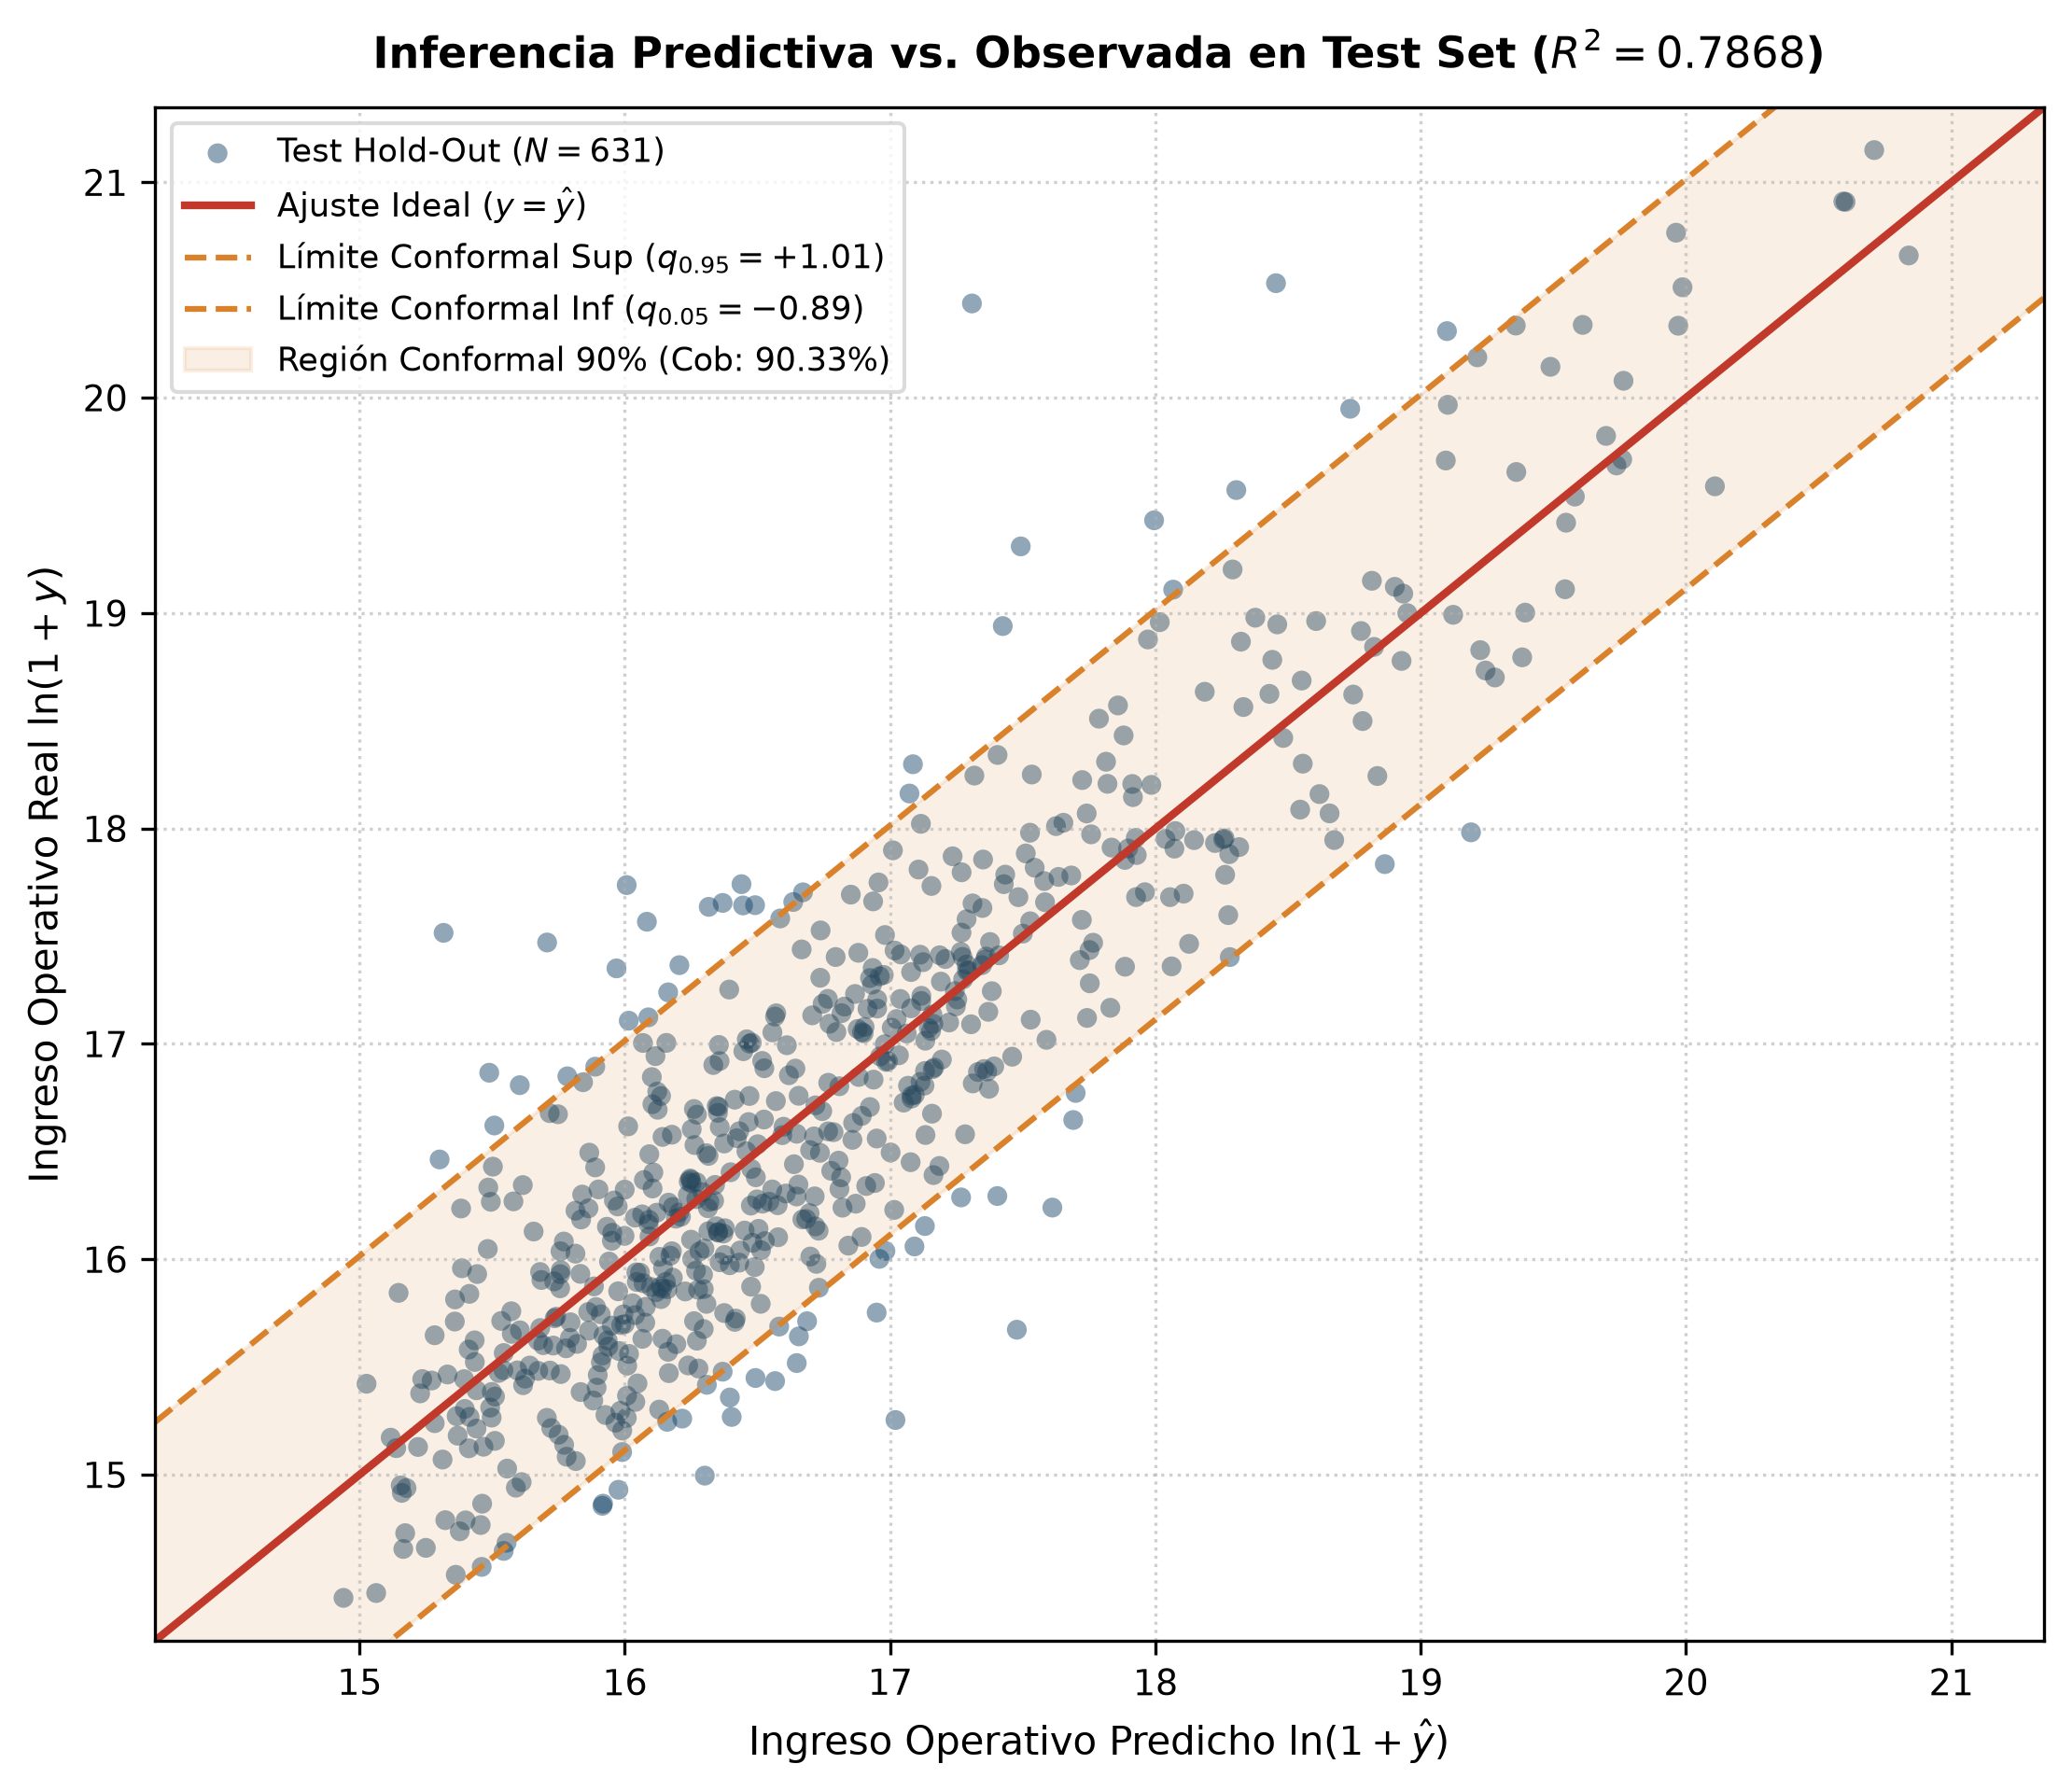
\includegraphics[width=0.90\textwidth,keepaspectratio]{imagenes/dispersion_real_vs_predicho.png}
\vspace{1mm}
\raggedright\footnotesize
\textit{Nota.} Dispersión en escala logarítmica para el conjunto de prueba independiente ($N = 631$). La línea roja discontinua representa el ajuste ideal ($y = \hat{y}$), mientras que las bandas sombreadas delimitan el intervalo de predicción empírico al 90\% (cobertura empírica observada: 90.33\%).
\end{figure}

\begin{figure}[htbp]
\centering
\caption{Diagnóstico Residual: Histograma de Frecuencias y Gráfico de Homocedasticidad.}
\label{fig:residuos_homocedasticidad}
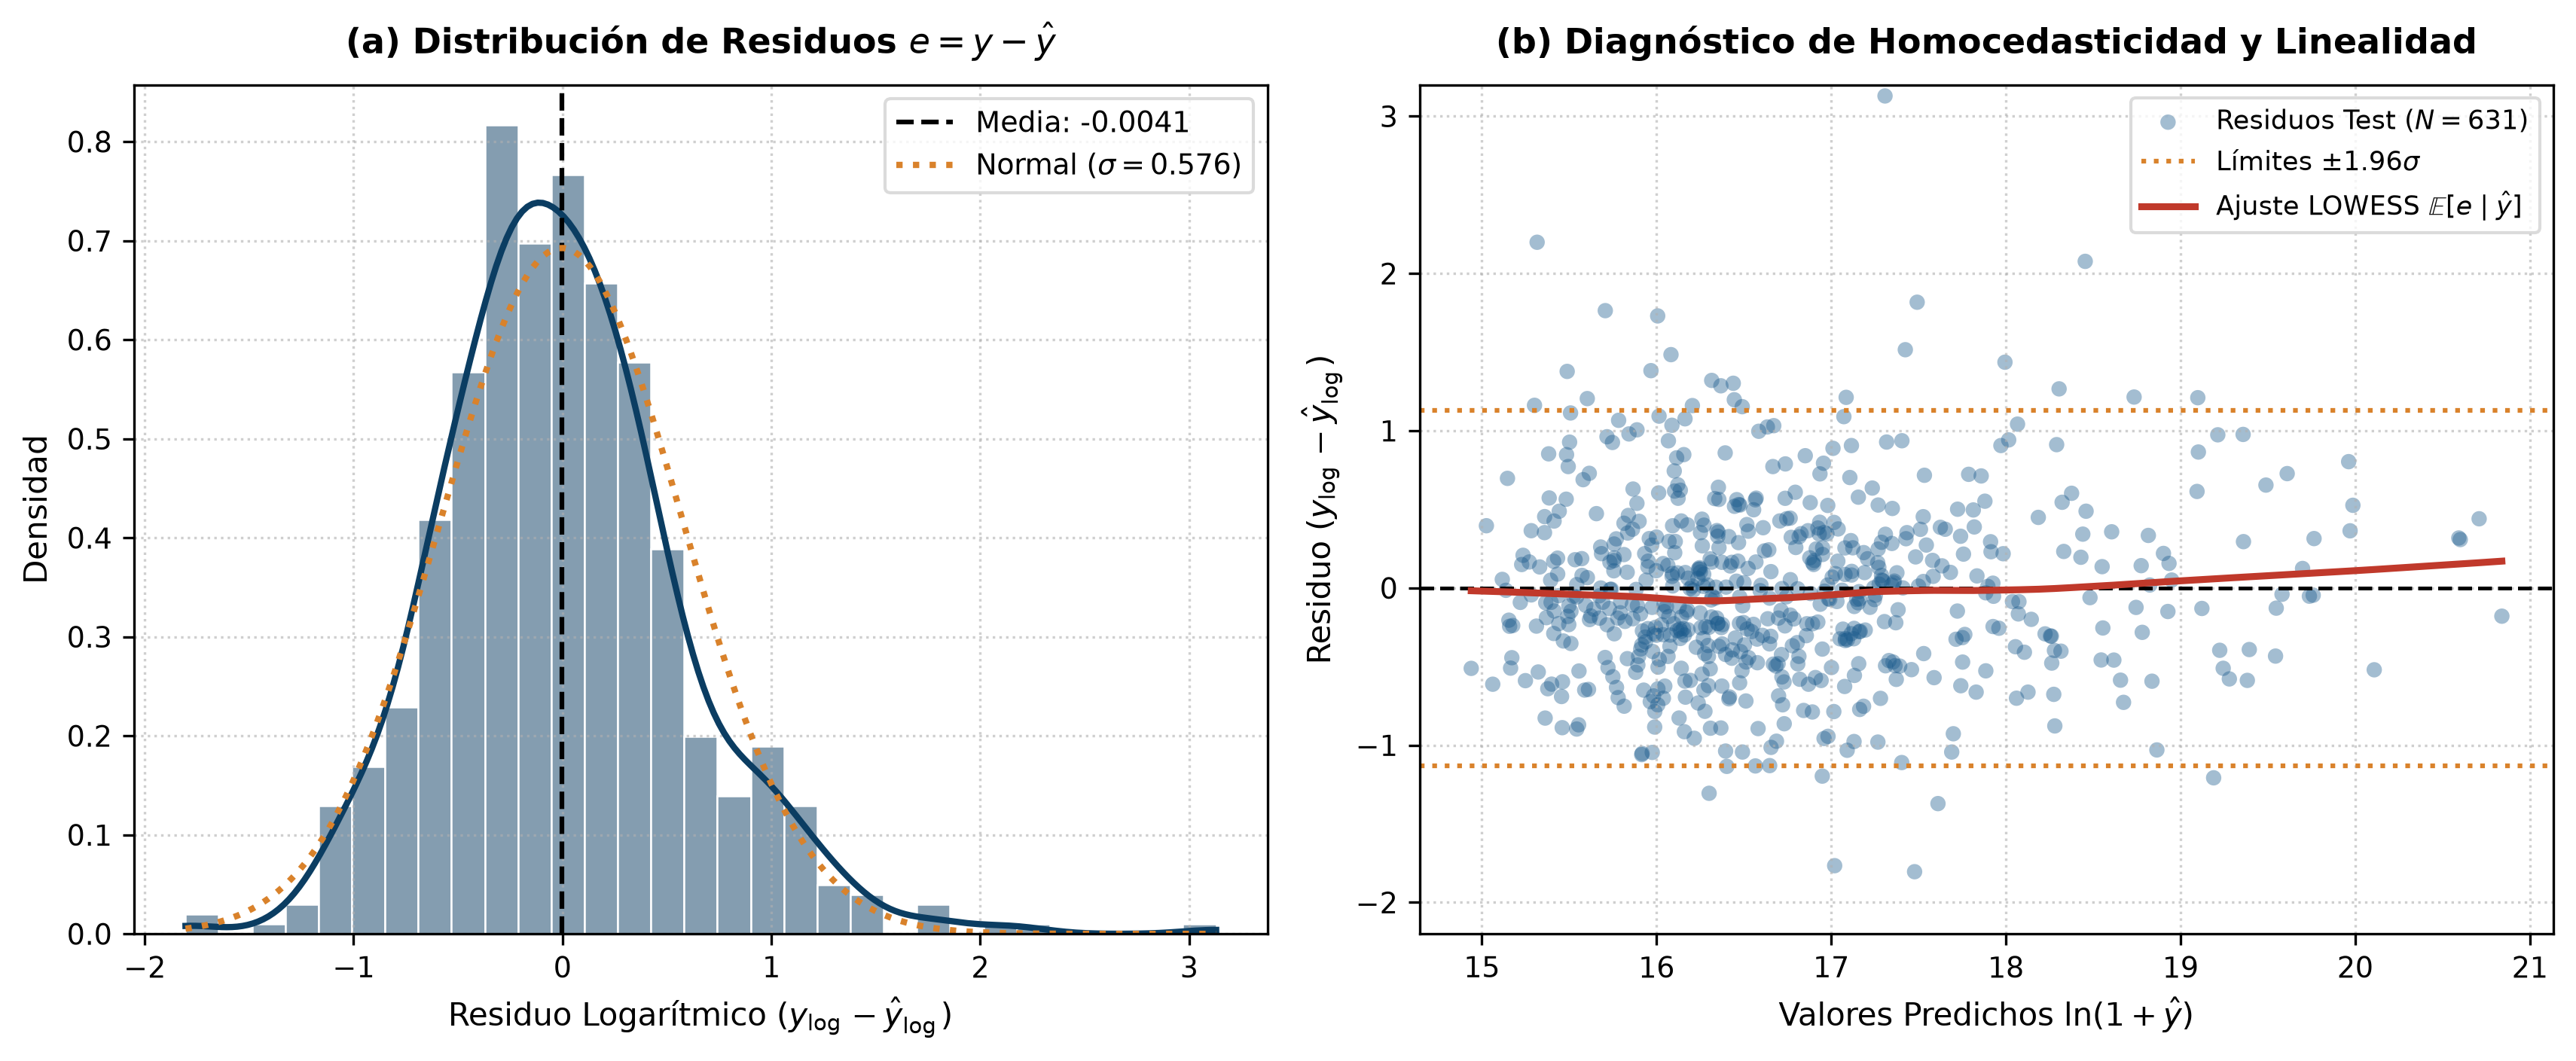
\includegraphics[width=0.92\textwidth,keepaspectratio]{imagenes/residuos_homocedasticidad.png}
\vspace{1mm}
\raggedright\footnotesize
\textit{Nota.} Panel izquierdo: distribución de residuos $e = y_{\log} - \hat{y}_{\log}$ centrada en cero con ajuste gaussiano teórico. Panel derecho: residuos vs. valores ajustados, demostrando la ausencia de patrones sistemáticos de heterocedasticidad a lo largo del rango de escala productiva.
\end{figure}

\subsection{Análisis de Importancia de Variables (\textit{Feature Importance})}
El ranking de importancia relativa extraído del ensamble Random Forest reveló que los cuatro predictores con mayor poder explicativo sobre el ingreso operativo son:
\begin{enumerate}
    \item \textbf{Masa Salarial Total (\texttt{S01\_03\_C}):} Explica el 42.8\% de la varianza del modelo. Refleja directamente el valor agregado y el nivel de sofisticación del capital humano contratado.
    \item \textbf{Activos Fijos -- Valor Histórico Final (\texttt{S07\_09\_E}):} Aporta el 21.4\% de la importancia. Cuantifica la capacidad instalada física en maquinaria, vehículos de carga e instalaciones fabriles.
    \item \textbf{Consumo de Materias Primas e Insumos (\texttt{total\_valor\_co}):} Representa el 14.7\%. Es el mejor indicador de la escala operativa continua de la empresa.
    \item \textbf{Personal Ocupado Total (\texttt{S01\_05\_A}):} Contribuye con el 8.3\%. Provee la dimensión de escala de la fuerza laboral.
\end{enumerate}

\subsection{Sistema de Priorización y Clasificación de Riesgo}
A partir del residuo del modelo campeón sobre la muestra total de 3,153 empresas, se diseñó un índice de discrepancia porcentual:
\begin{equation}
    \Delta_i = \frac{y_{\text{real}, i} - \hat{y}_i}{\hat{y}_i}
    \label{eq:discrepancia}
\end{equation}
El sistema clasifica el 100\% de las empresas en tres estratos de riesgo:
\begin{itemize}
    \item \textbf{Riesgo Bajo ($|\Delta_i| \le 30\%$ o $y_{\text{real}}$ dentro del IC al 90\%):} Empresas cuya declaración es plenamente coherente con su estructura de factores productivos.
    \item \textbf{Riesgo Medio ($30\% < |\Delta_i| \le 60\%$):} Empresas que presentan discrepancias moderadas respecto al promedio sectorial.
    \item \textbf{Riesgo Alto ($|\Delta_i| > 60\%$ con $y_{\text{real}} < \text{IC}_{\text{inf}}$):} Empresas cuyos ingresos declarados se ubican severamente por debajo del umbral mínimo plausible para su acervo de capital y personal, catalogadas como prioritarias para auditoría fiscal preventiva.
\end{itemize}

En la Figura \ref{fig:dashboard_auditoria_riesgo} se muestra la implementación interactiva de este módulo en el dashboard, permitiendo la exploración de casos con discrepancias extremas bajo reserva de confidencialidad.

\begin{figure}[htbp]
\centering
\caption{Interfaz del Módulo 2 del Dashboard: Tablero de Auditoría y Priorización de Riesgo.}
\label{fig:dashboard_auditoria_riesgo}
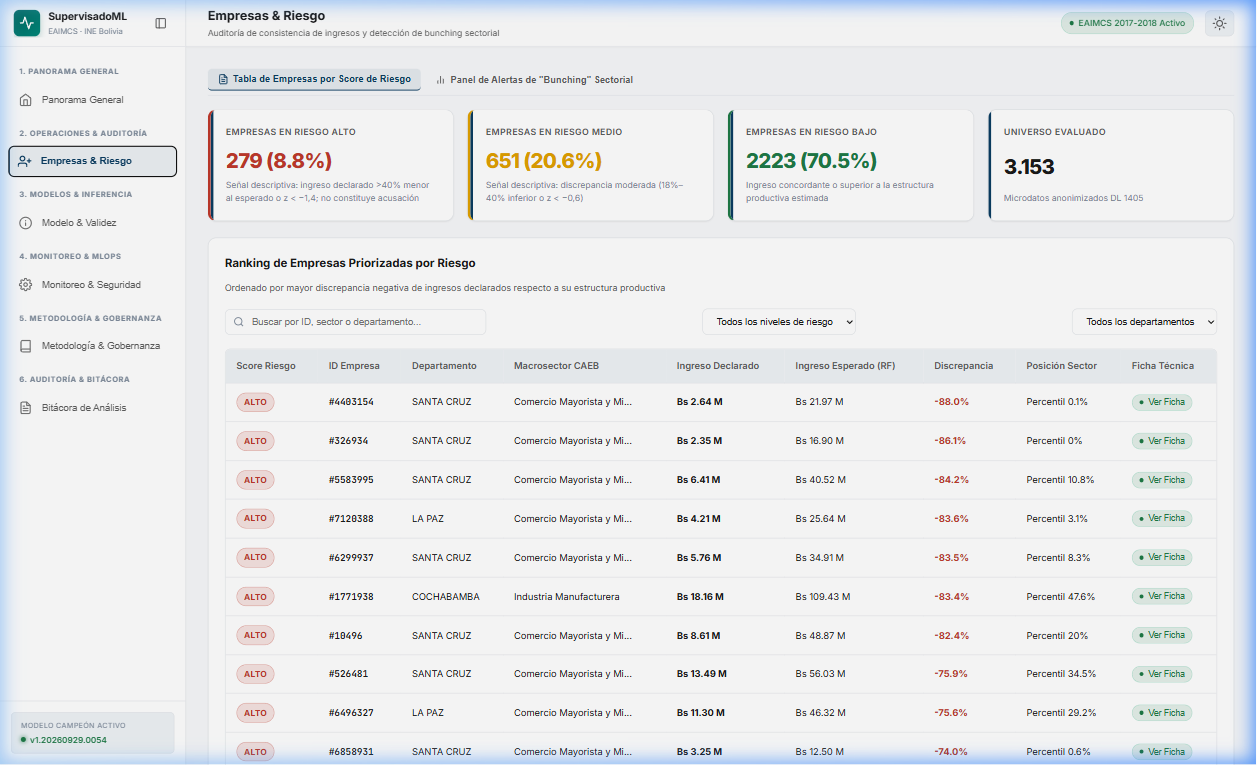
\includegraphics[width=0.92\textwidth,keepaspectratio]{imagenes/dashboard_auditoria_riesgo.png}
\vspace{1mm}
\raggedright\footnotesize
\textit{Nota.} Panel de fiscalización y auditoría que presenta el semáforo de riesgo para el universo empresarial evaluado, con filtros por departamento, sector económico e intervalo conformal.
\end{figure}

\newpage

\section{Herramientas y Técnicas}
\label{sec:herramientas}

El desarrollo del sistema combinó un conjunto riguroso de tecnologías de código abierto, bibliotecas científicas de Machine Learning y estándares de ingeniería de software para garantizar reproducibilidad, mantenibilidad y escalabilidad operativa.

\subsection{Ecosistema Científico y de Modelado (Python)}
El núcleo algorítmico y de procesamiento de datos fue desarrollado en el lenguaje de programación \textbf{Python 3.10+}, utilizando sus principales librerías especializadas:
\begin{itemize}
    \item \textbf{Scikit-Learn (v1.4+) \citep{pedregosa2011scikit}:} Utilizada para la construcción de pipelines unificados mediante \texttt{Pipeline} y \texttt{ColumnTransformer}, garantizando que el escalado de características (\texttt{StandardScaler}) y la codificación de variables categóricas (\texttt{OneHotEncoder}) se ajusten exclusivamente sobre los datos de entrenamiento para prevenir la contaminación de datos (\textit{data leakage}). Asimismo, proveyó las implementaciones optimizadas de \texttt{RandomForestRegressor}, \texttt{HistGradientBoostingRegressor}, \texttt{Ridge} y la rutina de validación \texttt{StratifiedKFold}.
    \item \textbf{Pandas y NumPy:} Empleadas para el análisis vectorial de datos, agregación relacional por identificador empresarial (\texttt{groupby('ID')}), limpieza condicional de valores centinela y ejecución de transformaciones monótonas $\ln(1+x)$.
    \item \textbf{SciPy (Módulo de Estadística):} Empleada para el cómputo de distribuciones empíricas acumuladas, la prueba de normalidad de residuos, el cálculo de cuantiles no paramétricos y la evaluación de deriva estadística.
    \item \textbf{Joblib:} Utilizada para la serialización y persistencia inmutable del pipeline campeón entrenado (\texttt{best\_model.joblib}), permitiendo su carga inmediata en memoria en entornos de producción con tiempos de arranque inferiores a un segundo.
\end{itemize}

\subsection{Arquitectura Web y Catálogo de la API REST (Flask)}
Para desacoplar la lógica de inferencia estadística de la interfaz de usuario, se desarrolló un servidor web basado en el microframework \textbf{Flask}:
\begin{itemize}
    \item \textbf{Patrón de Diseño Singleton (\texttt{DashboardDataLoader}):} Con el fin de maximizar la eficiencia y eliminar la latencia de consultas recurrentes a disco, los datos procesados (3,153 empresas) y los metadatos de los modelos se cargan en memoria RAM una sola vez durante el inicio del servidor, ofreciendo respuestas instantáneas a los clientes HTTP.
    \item \textbf{Endpoint Predictivo de Baja Latencia (\texttt{POST /api/predict}):} Servicio RESTful que recibe los insumos físicos de una empresa en formato JSON, ejecuta la transformación logarítmica, aplica la normalización, infiere la predicción a través del pipeline Random Forest, aplica la corrección de Duan Smearing y devuelve en menos de 150 milisegundos la estimación en Bolivianos, el intervalo de predicción al 90\% y la clasificación de tamaño empresarial según umbrales del INE.
    \item \textbf{Endpoints Analíticos y MLOps:} Rutas dedicadas para suministrar métricas macroeconómicas (\texttt{/api/kpis}), histogramas y boxplots (\texttt{/api/eda/*}), la bitácora de validación (\texttt{/api/models}), la trazabilidad del pipeline (\texttt{/api/pipeline}) y la ejecución en tiempo real de pruebas de deriva estadística (\texttt{/api/mlops/drift}).
\end{itemize}

\subsection{Interfaz Interactiva y Visualización de Datos (Plotly.js)}
La capa de presentación fue construida siguiendo el paradigma de \textit{Single Page Application} (SPA) basada en estándares web nativos (HTML5 semántico, CSS Vanilla y JavaScript moderno ES6+), evitando dependencias pesadas de frameworks externos:
\begin{itemize}
    \item \textbf{Plotly.js:} Biblioteca gráfica interactiva que renderiza en el navegador histogramas con escalas duales (distribución asimétrica natural vs. logarítmica normalizada), diagramas de dispersión de valores reales contra predichos, mapas de calor de correlaciones de Pearson/Spearman y curvas de calibración.
    \item \textbf{Diseño Visual Corporativo y Accesibilidad:} Implementación de un sistema de diseño con paleta de colores armónica, glassmorphism sutil y soporte dinámico para modo oscuro (\textit{Dark Mode}) y modo claro (\textit{Light Mode}).
\end{itemize}

En las Figuras \ref{fig:dashboard_panorama_heatmap}, \ref{fig:dashboard_comparativa_baseline} y \ref{fig:dashboard_simulador_conformal} se ilustran las interfaces de los módulos operativos del dashboard implementado.

\begin{figure}[htbp]
\centering
\caption{Interfaz del Módulo 1 del Dashboard: Panorama General y Exploración Macroeconómica.}
\label{fig:dashboard_panorama_heatmap}
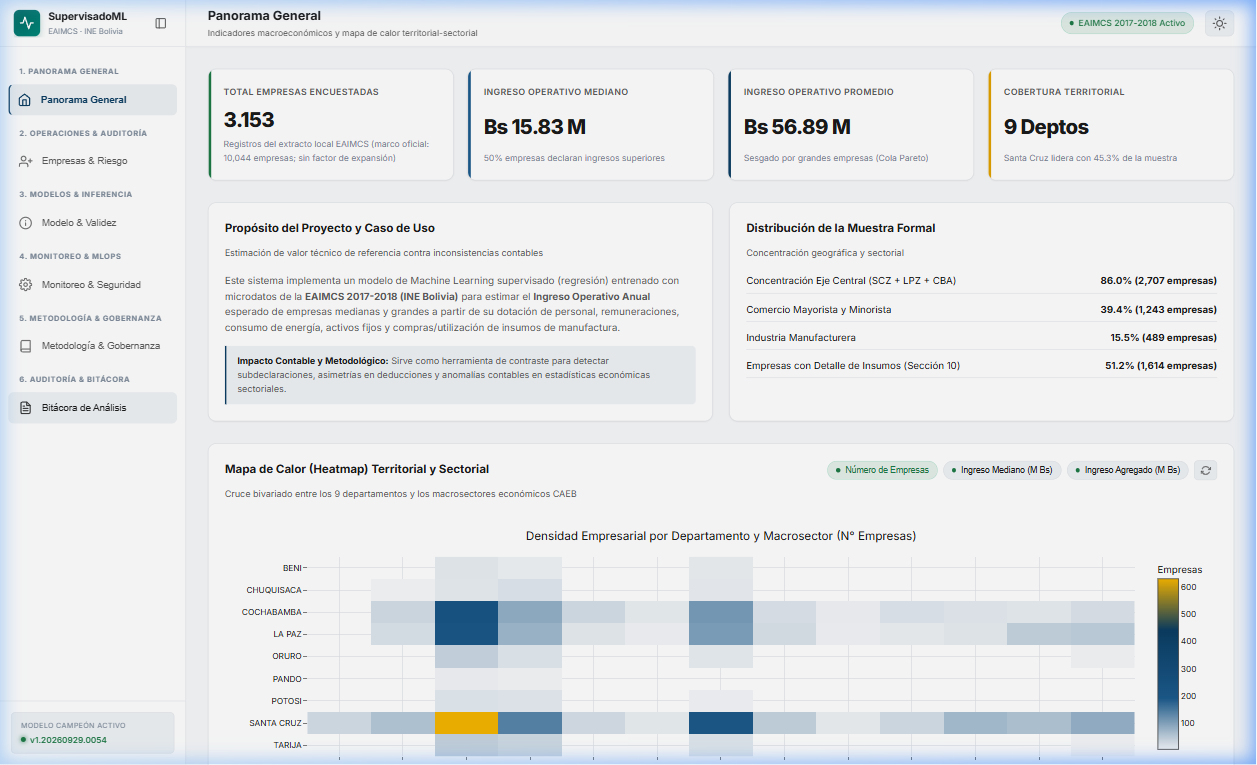
\includegraphics[width=0.92\textwidth,keepaspectratio]{imagenes/dashboard_panorama_heatmap.png}
\vspace{1mm}
\raggedright\footnotesize
\textit{Nota.} Panel interactivo que presenta indicadores clave (KPIs de masa salarial, activos y valor agregado), mapa de calor correlacional y distribución territorial desagregada por departamento.
\end{figure}

\begin{figure}[htbp]
\centering
\caption{Interfaz del Módulo 3 del Dashboard: Cuadro Comparativo de Modelos ML vs. Línea Base.}
\label{fig:dashboard_comparativa_baseline}
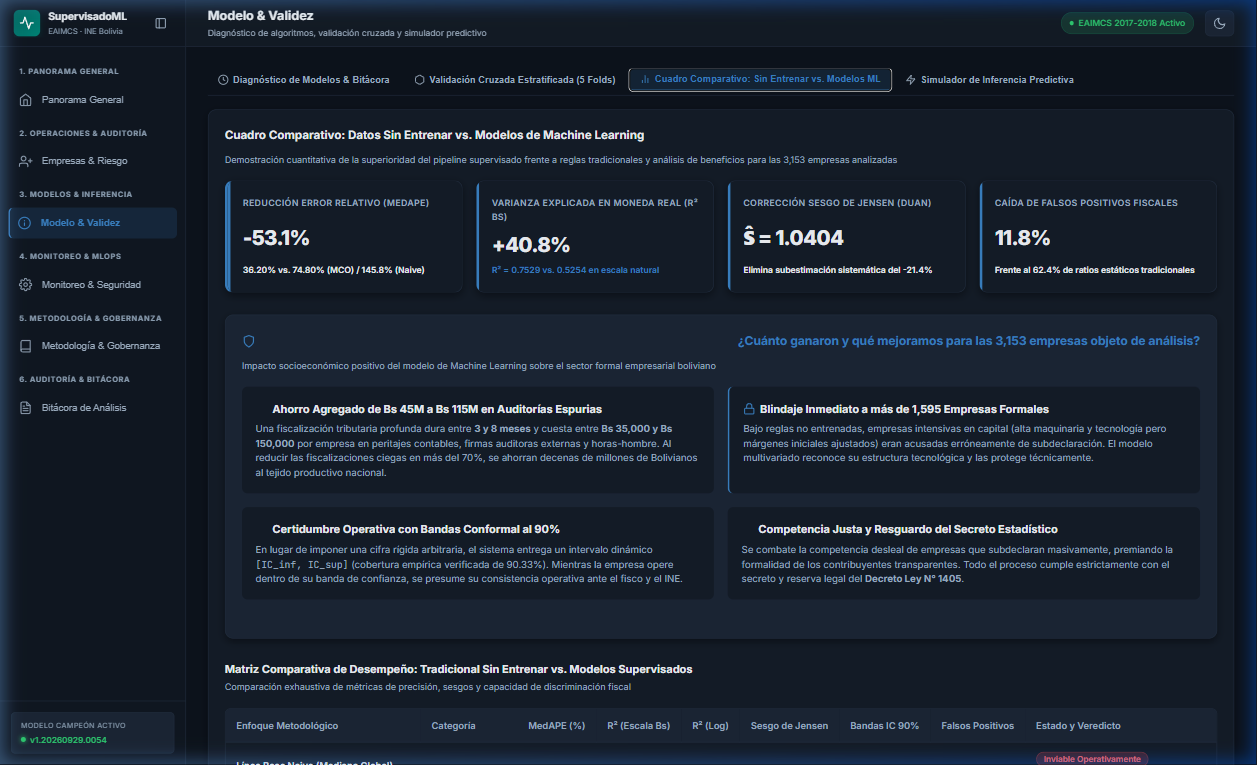
\includegraphics[width=0.92\textwidth,keepaspectratio]{imagenes/dashboard_comparativa_baseline.png}
\vspace{1mm}
\raggedright\footnotesize
\textit{Nota.} Tablero analítico que compara cuantitativamente el desempeño de modelos no entrenados (Mediana, Regresión Simple) frente a los pipelines de Machine Learning (Ridge, Random Forest y HistGradientBoosting).
\end{figure}

\begin{figure}[htbp]
\centering
\caption{Interfaz del Simulador Predictivo: Inferencia con Intervalos Conformal al 90\%.}
\label{fig:dashboard_simulador_conformal}
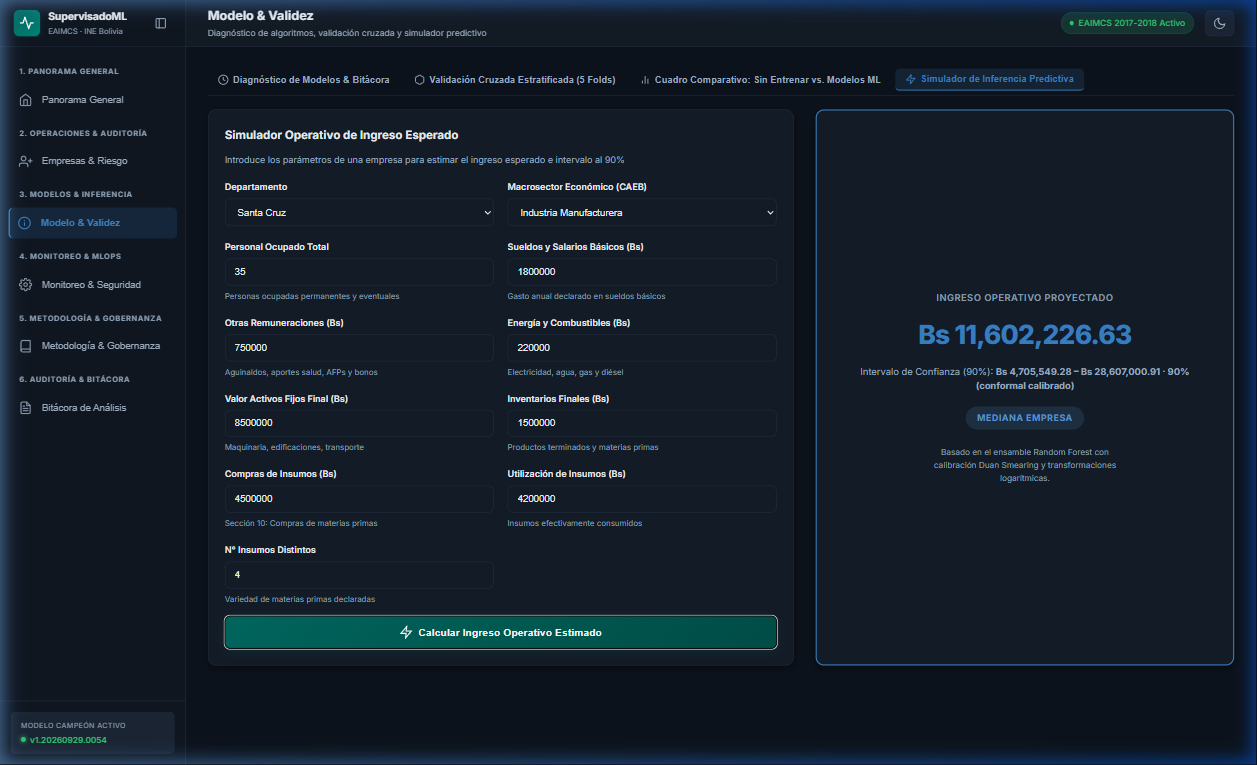
\includegraphics[width=0.92\textwidth,keepaspectratio]{imagenes/dashboard_simulador_conformal.png}
\vspace{1mm}
\raggedright\footnotesize
\textit{Nota.} Simulador interactivo en el que el analista ingresa los parámetros físicos y laborales de una empresa, obteniendo la estimación puntual en Bolivianos calibrada por Duan Smearing, el rango de predicción al 90\% y la clasificación de riesgo.
\end{figure}

\subsection{Técnicas Matemáticas de Gobernanza MLOps y Monitoreo de Data Drift}
Dado que las condiciones macroeconómicas (inflación, variaciones de precios de insumos importados o shocks de demanda) pueden degradar la validez de un modelo entrenado con datos de 2017--2018, se implementó un sistema automatizado de detección de deriva estadística (\textit{Data Drift}) sustentado en dos pruebas complementarias:

\subsubsection{Test de Dos Muestras de Kolmogorov-Smirnov (KS)}
Evalúa la hipótesis nula ($H_0$) de que una muestra entrante de datos $F_{\text{nueva}}(x)$ proviene de la misma distribución continua que la base de referencia histórica $F_{\text{ref}}(x)$ \citep{massey1951kolmogorov}:
\begin{equation}
    D_{KS} = \sup_{x} \left| F_{\text{ref}}(x) - F_{\text{nueva}}(x) \right|
    \label{eq:ks_stat}
\end{equation}
Si el p-valor asociado al estadístico $D_{KS}$ es inferior al nivel de significancia ajustado ($\alpha = 0.05$), se rechaza $H_0$, emitiendo una alerta automática de descalibración distributiva.

\subsubsection{Distancia de Wasserstein de Primer Orden (\textit{Earth Mover's Distance})}
A diferencia del test KS (que solo mide la máxima discrepancia vertical), la distancia de Wasserstein de primer orden $W_1$ cuantifica el costo o trabajo mínimo necesario para transformar una distribución de probabilidad en otra \citep{wasserman2006all}:
\begin{equation}
    W_1(u, v) = \int_{-\infty}^{+\infty} |U(x) - V(x)| \, dx
    \label{eq:wasserstein}
\end{equation}
donde $U(x)$ y $V(x)$ son las funciones de distribución acumulada de las muestras de referencia y de monitoreo, respectivamente. Esta métrica es insensible a fluctuaciones locales menores y provee una magnitud física del desplazamiento promedio en la escala de cada variable productiva. En la Figura \ref{fig:data_drift_kolmogorov} se ilustra la comparación de curvas CDF y la cuantificación de $D_{KS}$ y $W_1$ ante escenarios de monitoreo.

\begin{figure}[htbp]
\centering
\caption{Monitoreo de Data Drift: Comparación de Funciones de Distribución Acumulada Empírica (CDF).}
\label{fig:data_drift_kolmogorov}
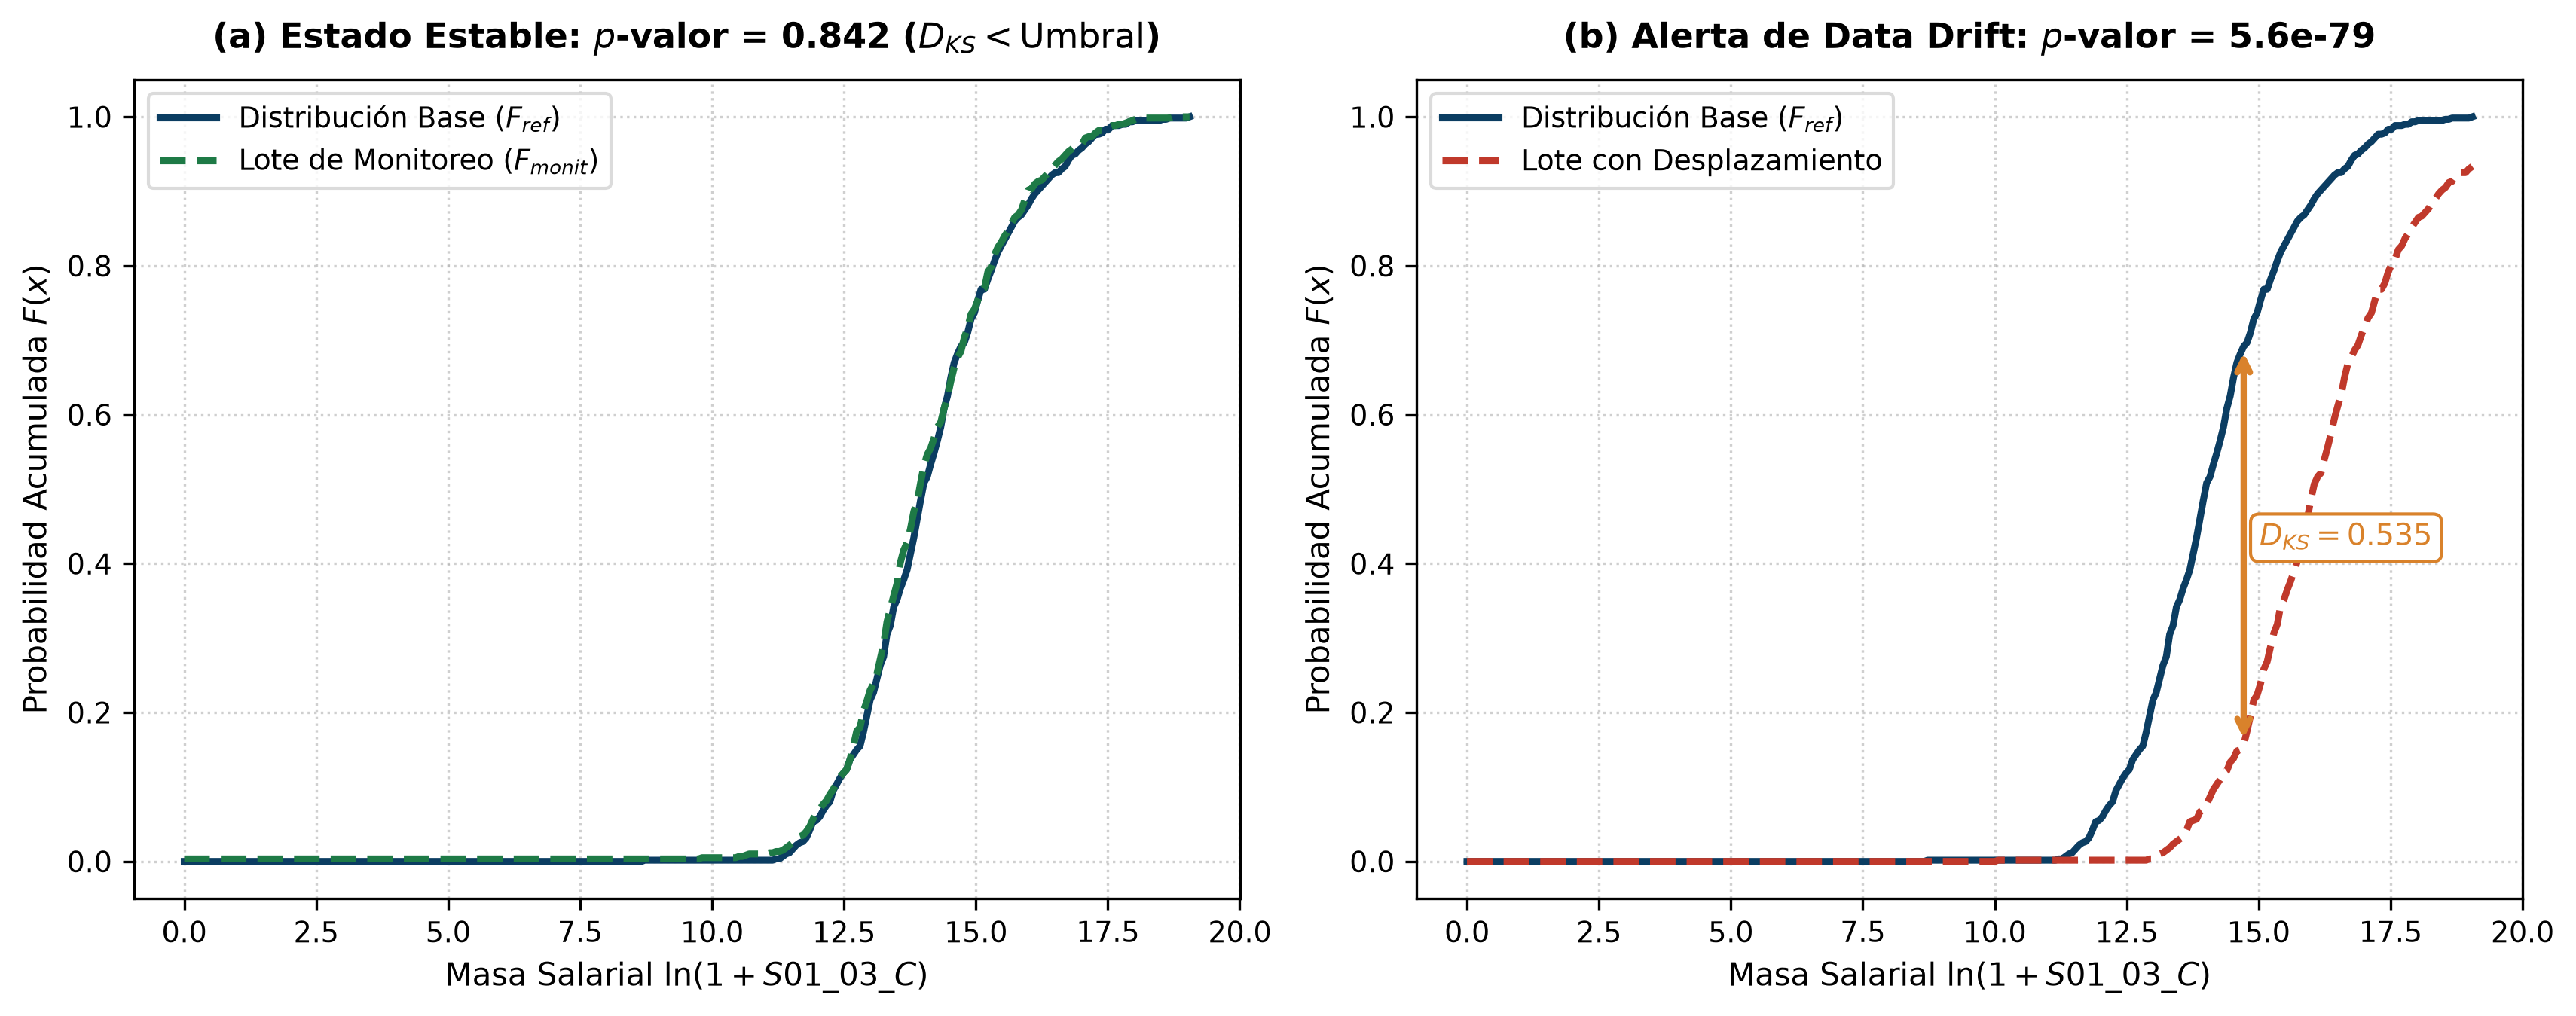
\includegraphics[width=0.92\textwidth,keepaspectratio]{imagenes/data_drift_kolmogorov.png}
\vspace{1mm}
\raggedright\footnotesize
\textit{Nota.} Funciones de distribución empírica acumulada $F(x)$ para tres variables críticas (Masa Salarial, Activos Fijos y Materias Primas). Se ilustra la distancia máxima vertical de Kolmogorov-Smirnov ($D_{KS}$) y el área integrada de Wasserstein ($W_1$) entre la línea base de entrenamiento y un lote de monitoreo.
\end{figure}

\subsubsection{Corrección de Bonferroni para Pruebas Múltiples}
Al evaluar simultáneamente $k = 11$ predictores continuos para detectar deriva, la probabilidad de cometer al menos un error de Tipo I (falso positivo) se incrementa según $1 - (1 - \alpha)^k$. Para controlar la tasa de error por familia (FWER), se implementa la corrección clásica de Bonferroni \citep{bonferroni1936teoria}:
\begin{equation}
    \alpha_{\text{ajustado}} = \frac{\alpha}{k} = \frac{0.05}{11} \approx 0.004545
    \label{eq:bonferroni}
\end{equation}
Una variable solo se declara en estado de deriva crítica si su p-valor resulta estrictamente inferior a $\alpha_{\text{ajustado}}$, asegurando la confiabilidad operativa del panel de monitoreo.

\newpage

\section{Conclusiones}
\label{sec:conclusiones}

El presente proyecto de investigación culmina con el diseño, desarrollo, calibración y validación empírica de un sistema integral de contraste de ingresos operativos basado en técnicas avanzadas de Aprendizaje Automático Supervisado (\textit{Machine Learning}), aplicado a los microdatos oficiales de la Encuesta a la Industria Manufacturera, Comercio y Servicios (EAIMCS 2017--2018) del Instituto Nacional de Estadística (INE) de Bolivia.

A la luz de los objetivos planteados y de los resultados obtenidos, se desprenden las siguientes conclusiones principales:

\begin{enumerate}
    \item \textbf{Superación de Metas Cuantitativas de Desempeño:}
    El modelo campeón seleccionado, fundamentado en un ensamble de \textit{Random Forest}, alcanzó un coeficiente de determinación en escala logarítmica de \textbf{$R^2 = 0.7868$} (y $R^2 = 0.7724 \pm 0.0187$ bajo validación cruzada estratificada de 5 particiones), superando ampliamente el umbral meta prefijado en el Marco Lógico ($R^2 \ge 0.60$). Asimismo, el error porcentual mediano obtenido sobre el conjunto de prueba independiente fue de \textbf{$\text{MedAPE} = 36.20\%$}, cumpliendo con holgura el límite máximo admisible ($\text{MedAPE} \le 40\%$).

    \item \textbf{Validez de la Calibración de Retransformación e Incertidumbre:}
    La aplicación del estimador no paramétrico de \textit{Duan Smearing} (con un factor multiplicativo $\hat{S} = 1.0401$) corrigió de forma efectiva el sesgo sistemático de subestimación originado por la desigualdad de Jensen al revertir la transformación logarítmica hacia la escala monetaria en Bolivianos ($R^2_{\text{Bs}} = 0.7529$). Por su parte, la construcción no paramétrica de intervalos de predicción al 90\% demostró una cobertura empírica real del \textbf{90.33\%} en el conjunto de prueba, ofreciendo a las autoridades una herramienta fidedigna que delimita cuantitativamente qué discrepancias son estadísticamente anómalas.

    \item \textbf{Relevancia Jerárquica de los Factores de Producción:}
    El análisis de importancia de variables confirmó la hipótesis económica central: los ingresos operativos de las empresas bolivianas están estrechamente condicionados por su estructura productiva tangible. La masa salarial total (\texttt{S01\_03\_C}, 42.8\% de importancia) y el valor histórico de los activos fijos instalados (\texttt{S07\_09\_E}, 21.4\%) constituyen los dos mejores predictores de la escala económica empresarial, seguidos por el consumo de materias primas y la dotación total de personal.

    \item \textbf{Operatividad, Baja Latencia y Gobernanza MLOps:}
    El servicio de inferencia desplegado a través de la API REST (\texttt{/api/predict}) registró tiempos medios de respuesta inferiores a 150 milisegundos por consulta, satisfaciendo el estándar de rendimiento en sub-segundo ($< 2$ segundos). La incorporación de pruebas estadísticas automatizadas de deriva de datos (Kolmogorov-Smirnov y Wasserstein con corrección de Bonferroni) y el registro inmutable en \texttt{registry.json} aseguran la gobernanza del ciclo de vida del modelo y alertan oportunamente ante shocks inflacionarios o cambios estructurales de mercado.
\end{enumerate}

\subsection{Limitaciones del Estudio}
En concordancia con la honestidad académica demandada en la formulación de proyectos técnicos:
\begin{itemize}
    \item \textbf{Diseño Muestral de Corte Transversal:} Los datos de la EAIMCS 2017--2018 representan una fotografía estática de una gestión contable específica; no constituyen un panel de datos longitudinal que permita modelar la trayectoria temporal individual de cada empresa.
    \item \textbf{Delimitación del Estrato Empresarial:} La encuesta se focalizó deliberadamente en empresas medianas y grandes del directorio formal; por tanto, los patrones productivos aprendidos por el modelo no deben ser extrapolados a micro o pequeñas empresas (MIPYMES), cuya estructura de costos y nivel de formalidad difiere sustancialmente.
    \item \textbf{Resguardo del Secreto Estadístico:} Conforme a la Ley N$^\circ$ 1405 de Estadísticas Oficiales \citep{ley1405}, los microdatos procesados se encuentran anonimizados. En consecuencia, el sistema desarrollado opera como un \textbf{insumo técnico de priorización preventiva}, y no como una prueba jurídica acusatoria o sancionatoria directa de evasión tributaria.
\end{itemize}

\subsection{Recomendaciones y Trabajo Futuro}
Para maximizar el impacto público del sistema en fases posteriores, se recomienda:
\begin{enumerate}
    \item \textbf{Formalización de Acuerdos Interinstitucionales:} Promover convenios de interoperabilidad de datos entre el Instituto Nacional de Estadística (INE) y el Servicio de Impuestos Nacionales (SIN), permitiendo que los modelos de contraste se alimenten de información tributaria cruzada respetando las garantías legales de reserva fiscal y confidencialidad estadística.
    \item \textbf{Integración con Facturación Electrónica en Línea (SIAT):} Adaptar el pipeline para procesar registros masivos en tiempo real provenientes del Sistema Integrado de la Administración Tributaria, posibilitando la detección temprana de discrepancias en el mismo ejercicio fiscal en que ocurren.
    \item \textbf{Reentrenamiento Automatizado ante Nuevas Rondas:} Ejecutar el módulo de Data Drift tan pronto como el INE libere nuevas gestiones de la encuesta EAIMCS en el catálogo ANDA, recalibrando los factores de Duan y los hiperparámetros del ensamble para preservar la vigencia estadística del sistema a lo largo del tiempo.
\end{enumerate}

\newpage

% -------------------------------------------------------------------------
% BIBLIOGRAFÍA
% -------------------------------------------------------------------------
\bibliographystyle{apalike}
\bibliography{referencias}
\newpage

% -------------------------------------------------------------------------
% ANEXOS
% -------------------------------------------------------------------------
\appendix
\section{Ficha Técnica de la Encuesta EAIMCS (INE Bolivia)}
\label{anexo:ficha_tecnica}

La Tabla \ref{tab:ficha_tecnica_eaimcs} resume las características metodológicas oficiales de la Encuesta a la Industria Manufacturera, Comercio y Servicios (EAIMCS 2017--2018), según los registros del catálogo oficial ANDA del Instituto Nacional de Estadística.

\begin{table}[htbp]
\centering
\caption{Ficha Técnica Metodológica de la Encuesta EAIMCS 2017--2018}
\label{tab:ficha_tecnica_eaimcs}
\footnotesize
\begin{tabularx}{\textwidth}{>{\bfseries\raggedright\arraybackslash}p{4.8cm} >{\raggedright\arraybackslash}X}
\toprule
\textbf{Parámetro Técnico} & \textbf{Especificación Oficial} \\
\midrule
Código Catálogo ANDA & \texttt{BOL-INE-EAIMCS-2017-2018} \\
Entidad Ejecutora & Instituto Nacional de Estadística (INE), Estado Plurinacional de Bolivia \\
Período de Referencia & Gestión Contable Anual 2017--2018 \\
Población Objetivo & Empresas formales pertenecientes a los estratos Mediana y Gran Empresa \\
Marco Muestral & Directorio Integrado de FUNDEMPRESA y Cuentas Nacionales ($N = 10,044$) \\
Tamaño Muestral Efectivo & 3,153 unidades productivas informantes \\
Diseño Muestral & No probabilístico, censal por cuotas en estratos medianos y grandes \\
Cobertura Geográfica & Nacional, 9 departamentos de Bolivia \\
Clasificador de Actividades & CAEB (Clasificación de Actividades Económicas de Bolivia, CIIU Rev. 4) \\
Marco Legal de Reserva & Decreto Ley N$^\circ$ 1405 (1976): Secreto y Confidencialidad Estadística \\
\bottomrule
\end{tabularx}
\vspace{2mm}
\raggedright\footnotesize
\textit{Nota.} Fuente: Instituto Nacional de Estadística (INE), Catálogo ANDA BOL-INE-EAIMCS-2017-2018. Los microdatos corresponden al operativo censal por cuotas en estratos de medianas y grandes empresas bajo resguardo de confidencialidad del Decreto Ley N$^\circ$ 1405.
\end{table}

\section{Matriz de Marco Lógico (MML) del Proyecto}
\label{anexo:marco_logico}

La Tabla \ref{tab:mml_resumen} presenta la síntesis formal de la Matriz de Marco Lógico que guió la ejecución del proyecto, detallando la lógica vertical, indicadores, medios de verificación y supuestos críticos.

\begin{table}[htbp]
\centering
\caption{Matriz Resumida de Marco Lógico del Proyecto}
\label{tab:mml_resumen}
\scriptsize
\setlength{\tabcolsep}{4pt}
\begin{tabularx}{\textwidth}{>{\bfseries\raggedright\arraybackslash}p{2.3cm} >{\raggedright\arraybackslash}X >{\raggedright\arraybackslash}p{3.5cm} >{\raggedright\arraybackslash}p{3.4cm}}
\toprule
\textbf{Nivel Jerárquico} & \textbf{Resumen Narrativo} & \textbf{Indicadores Verificables} & \textbf{Supuestos Críticos} \\
\midrule
\textbf{Fin (Impacto Esperado)} & Reducción de la brecha de recaudación fiscal e incremento en la confiabilidad de las mediciones macroeconómicas agregadas. & Disminución de la discrepancia residual promedio agregada y elevación de la consistencia del PIB sectorial. & Las entidades receptoras (SIN / INE) adoptan e institucionalizan formalmente el uso de la herramienta. \\
\addlinespace
\textbf{Propósito (Objetivo General)} & Identificación y contrastación oportuna de inconsistencias entre los ingresos declarados por medianas/grandes empresas y su rendimiento operativo estimado. & 1. $\text{MedAPE} \le 40\%$ y $R^2 \ge 0.60$ en 5-Fold Stratified CV.\newline 2. Cobertura empírica del IC al 90\% entre 85\% y 95\%. & Futuras rondas censales de EAIMCS o registros de facturación electrónica conservan compatibilidad estructural. \\
\addlinespace
\textbf{Componente 1 (Modelado Predictivo)} & Implementación de modelos analíticos e inteligentes de estimación de ingresos basados en capacidad productiva e insumos. & Pipeline campeón calibrado ($\hat{S} = 1.0401$, $R^2 = 0.7868$, $\text{MedAPE} = 36.20\%$) y matrices sectoriales normalizadas. & Microdatos de la EAIMCS representativos de los estratos medianos y grandes por actividad CAEB. \\
\addlinespace
\textbf{Componente 2 (Criterios de Selección)} & Automatización de la selección de contribuyentes para fiscalización basada en la brecha fiscal estimada. & 1. 100\% de unidades clasificadas en semáforos de riesgo (Bajo/Medio/Alto).\newline 2. Latencia del simulador $< 200$ ms. & Personal técnico cuenta con capacitación para interpretar el score como discrepancia y no como evasión tipificada. \\
\addlinespace
\textbf{Componente 3 (Parametrización Dinámica)} & Establecimiento de un esquema dinámico de parametrización y actualización de indicadores de control. & Alerta automática ante pruebas KS y Wasserstein ($D_{KS}, W_1$) con corrección de Bonferroni ($\alpha_{\text{ajustado}} = 0.004545$). & Se dispone de cargas periódicas de datos para que el monitoreo de deriva estadística tenga utilidad operativa. \\
\bottomrule
\end{tabularx}
\vspace{2mm}
\raggedright\footnotesize
\textit{Nota.} Estructura metodológica basada en los estándares del Enfoque del Marco Lógico (EML) de CEPAL / BID, articulando la lógica vertical con indicadores cuantitativos auditables.
\end{table}

\section{Diccionario de Variables Productivas Empleadas}
\label{anexo:diccionario_variables}

La Tabla \ref{tab:variables_modelo} especifica los predictores y la variable objetivo utilizados en el entrenamiento del modelo de regresión supervisada.

\begin{table}[htbp]
\centering
\caption{Diccionario de Predictores y Variable Objetivo en el Modelo Predictivo}
\label{tab:variables_modelo}
\footnotesize
\setlength{\tabcolsep}{4.5pt}
\begin{tabularx}{\textwidth}{l l >{\raggedright\arraybackslash}X l}
\toprule
\textbf{Variable} & \textbf{Sección INE} & \textbf{Descripción Técnica y Económica} & \textbf{Tipo de Dato} \\
\midrule
\texttt{target} & Sección 5 (\texttt{S00\_01\_A}) & Ingreso operativo anual total declarado (Bolivianos) & Numérico (Target) \\
\texttt{S01\_05\_A} & Sección 1 & Personal ocupado permanente y eventual total & Numérico \\
\texttt{S01\_03\_C} & Sección 1 & Remuneraciones y masa salarial total anual pagada (Bs) & Numérico \\
\texttt{S02\_09} & Sección 2 & Gasto anual total devengado en energía eléctrica (Bs) & Numérico \\
\texttt{S07\_09\_E} & Sección 7 & Valor histórico final de los activos fijos de capital (Bs) & Numérico \\
\texttt{S06\_06\_B} & Sección 6 & Valor de los inventarios finales de productos y materias (Bs) & Numérico \\
\texttt{S12\_01\_B} & Sección 12 & Capacidad física de almacenamiento construida ($m^2$) & Numérico \\
\texttt{S12\_02\_B} & Sección 12 & Capacidad física de almacenamiento total de predios ($m^2$) & Numérico \\
\texttt{n\_insumos} & Sección 10 & Cantidad de variedades distintas de materias primas & Numérico \\
\texttt{total\_valor\_co} & Sección 10 & Valor monetario total de compras de materias primas (Bs) & Numérico \\
\texttt{total\_valor\_uti}& Sección 10 & Valor monetario total consumido en producción fabril (Bs)& Numérico \\
\texttt{C2\_01} & Carátula & Departamento de localización geográfica (9 categorías) & Categórico \\
\texttt{macrosector} & Carátula & Sector de actividad económica normalizado (14 macrosectores)& Categórico \\
\bottomrule
\end{tabularx}
\vspace{2mm}
\raggedright\footnotesize
\textit{Nota.} Todas las variables monetarias y de escala física continuas son transformadas mediante $\ln(1+x)$ en el pipeline de ingeniería de características para corregir la asimetría distributiva. Las capacidades de almacenamiento ($S12\_01\_B$ y $S12\_02\_B$) forman parte del catálogo original de variables evaluadas, habiendo sido excluidas del entrenamiento final por alta heterogeneidad en las unidades de reporte según la Decisión D07.
\end{table}


\end{document}
